\documentclass[a4paper,12pt,twoside]{report}
%\usepackage[utf8]{inputenc}
\usepackage[]{graphicx}

%\documentclass[10pt]{article}
\usepackage[margin=3cm]{geometry}
\usepackage{array, xcolor} %έσβησα το πακέτο bibentry
\usepackage{color,hyperref,url}
\usepackage{graphicx}

%================ΕΝΑΡΞΗ ΒΙΒΛΙΟΘΗΚΩΝ=========================

\setlength{\paperwidth}{21cm}          % Largura da página
\setlength{\paperheight}{29,7cm}       % Altura da página
\setlength{\textwidth}{15.5cm}         % Largura do texto
\setlength{\textheight}{24.6cm}        % Altura do texto
\setlength{\topmargin}{-1.0cm}         % Margem superior da página = 1 polegada + valor atribuição.
                                      % \setlenght{\topmargin}{0cm} dá 2.54cm de margem superior.
\setlength{\oddsidemargin}{0.46cm}   % Margem esquerda = 1 polegada + valor
\setlength{\evensidemargin}{0.46cm} 

% Προσοχή στο [cm-default], χωρίς αυτό μπορεί να μην λειτουργούν τα
% μαθηματικά σύμβολα σε ορισμένες εγκαταστάσεις του xelatex!
\usepackage[cm-default]{fontspec} % ίσως εμφανίσει πρόβλημα
\usepackage{xunicode}
\usepackage{xltxtra}

% Ελληνικό Hyphenation, αφαιρέστε το αν δεν έχετε εγκατεστημένο το xgreek.
\usepackage{xgreek}

% Μερικές γραμματοσειρές
\setromanfont{FreeSerif}
\setsansfont{FreeSans}
\setmonofont{FreeMono}

%% The amssymb package provides various useful mathematical symbols
% http://tex.stackexchange.com/questions/58098/what-are-all-the-font-styles-i-can-use-in-math-mode
\usepackage{amsmath,amsfonts,amsthm,amssymb}
\usepackage[mathscr]{euscript}

%\usepackage{mathtools}
\usepackage{calrsfs}

% Macros about theorems, definitions, examples
%\newcounter{chapter}
% Ιδέες από: http://tex.stackexchange.com/questions/82415/beamer-different-numbering-for-theorems-examples-definition-and-lemma
\theoremstyle{plain}
\newtheorem{thm}{Θεώρημα}[section] % reset theorem numbering for each chapter
\newtheorem{cor}{Πόρισμα}[section]

\theoremstyle{definition}
\newtheorem{defn}{Ορισμός}[section] % definition numbers are dependent on theorem numbers
\newtheorem{exmp}{Παράδειγμα}[section] % same for example numbers

\theoremstyle{remark}
\newtheorem*{rem}{Παρατήρηση}
\newtheorem*{note}{Σημείωση}

%% The lineno packages adds line numbers. Start line numbering with
%% \begin{linenumbers}, end it with \end{linenumbers}. Or switch it on
%% for the whole article with \linenumbers after \end{frontmatter}.
\usepackage{lineno}

%% Packages for the algorithm and pseudocode
\usepackage{algorithm}
\usepackage[noend]{algpseudocode}

%% Defining some helpful commands/abbreviations
%\DeclarePairedDelimiter\abs{\lvert}{\rvert}%
%\DeclarePairedDelimiter\norm{\lVert}{\rVert}%
%\DeclareMathOperator*{\argmin}{arg\,min}

%% Package for many columns
%\usepackage{multicol}

%% For inserting pictures inside the multicolumns
\usepackage{wrapfig}
\usepackage{multirow}

% Για να εμφανίσει την βιβλιογραφία ως αναφορές ή βιβλιογραφία
\renewcommand{\refname}{Αναφορές}
\renewcommand\bibname{Αναφορές}
%% Για έξυπνες αναφορές:
%%% http://tex.stackexchange.com/questions/35921/multiple-subequation-labels-in-one-ref

%% ΓΙα εισαγωγή κώδικα σε λατεχ. (δεν χρειάζεται, δες πιο πάνω)
% \usepackage{listings}
% \lstset{
%   basicstyle=\ttfamily,
%   mathescape
% }

%For inserting MATLAB code in latex
%\usepackage[framed,numbered,autolinebreaks,useliterate]{mcode}
% Gives error with "autolinebreaks" and "useliterate" and they don't seem to 
% be needed.
\usepackage[framed,numbered]{mcode}

%%% To use listings for code
\usepackage{listings}
\usepackage{color}

\definecolor{mygreen}{rgb}{0,0.6,0}
\definecolor{mygray}{rgb}{0.2,0.2,0.2}
\definecolor{mymauve}{rgb}{0.58,0,0.82}

\lstset{ %
  backgroundcolor=\color{white},   % choose the background color; you must add \usepackage{color} or \usepackage{xcolor}; should come as last argument
  basicstyle=\footnotesize,        % the size of the fonts that are used for the code
  breakatwhitespace=false,         % sets if automatic breaks should only happen at whitespace
  breaklines=true,                 % sets automatic line breaking
  captionpos=b,                    % sets the caption-position to bottom
  commentstyle=\color{mygreen},    % comment style
  deletekeywords={...},            % if you want to delete keywords from the given language
  escapeinside={\%*}{*)},          % if you want to add LaTeX within your code
  extendedchars=true,              % lets you use non-ASCII characters; for 8-bits encodings only, does not work with UTF-8
  frame=single,	                   % adds a frame around the code
  keepspaces=true,                 % keeps spaces in text, useful for keeping indentation of code (possibly needs columns=flexible)
  keywordstyle=\color{blue},       % keyword style
  language=Octave,                 % the language of the code
  morekeywords={*,...},           % if you want to add more keywords to the set
  numbers=left,                    % where to put the line-numbers; possible values are (none, left, right)
  numbersep=5pt,                   % how far the line-numbers are from the code
  numberstyle=\tiny\color{mygray}, % the style that is used for the line-numbers
  rulecolor=\color{black},         % if not set, the frame-color may be changed on line-breaks within not-black text (e.g. comments (green here))
  showspaces=false,                % show spaces everywhere adding particular underscores; it overrides 'showstringspaces'
  showstringspaces=false,          % underline spaces within strings only
  showtabs=false,                  % show tabs within strings adding particular underscores
  stepnumber=1,                    % the step between two line-numbers. If it's 1, each line will be numbered
  stringstyle=\color{mymauve},     % string literal style
  tabsize=2,	                   % sets default tabsize to 2 spaces
  title=\lstname                   % show the filename of files included with \lstinputlisting; also try caption instead of title
}

%%% Για το \uminus αντίστοιχο του \uplus
\makeatletter
\providecommand*{\uminus}{%
  \mathbin{%
    \mathpalette\@uminus{}%
  }%
}
\newcommand*{\@uminus}[2]{%
  \ooalign{%
    $\m@th#1\cup$\cr
    \hidewidth$\m@th#1\text{-}$\hidewidth
  }%
}
\makeatother
%%%%%%-------------------ΤΕΛΟΣ ΒΙΒΛΙΟΘΗΚΩΝ---------------------

\begin{document}

%%%%%%%%%%%%%%%%%%%%%%%%%%%%%%%%%%%%%%%%%%%%%%%%%%%%%%%%%%%%%%%%%%%%%%%%%%%%%%%%%%%%%%%%%
%%%%%%% 			CAPA DO TRABALHO ou Folha de rosto					 	 %%%%%%%%%%%%
%a. Folha de rosto, contendo os seguintes itens:							
%• Nome do aluno;
%• Nome do orientador e coorientador, se houver;
%• Data de início do Doutorado;
%• Se for bolsista, nome da agência financiadora e data de início da bolsa;
%%%%%%%%%%%%%%%%%%%%%%%%%%%%%%%%%%%%%%%%%%%%%%%%%%%%%%%%%%%%%%%%%%%%%%%%%%%%%%%%%%%%%

\begin{figure}
  \centering
  
\includegraphics[]{patrasLogo.jpg}
  \vspace*{0.3cm}
\end{figure}

\begin{center}
%{\large \rm \textbf {ΠΑΝΕΠΙΣΤΗΜΙΟ ΠΑΤΡΩΝ} \linebreak}
{\large \rm \textbf {ΤΜΗΜΑ ΜΑΘΗΜΑΤΙΚΩΝ} \linebreak}
{\large \rm \textbf {Μ.Δ.Ε. ΜΑΘΗΜΑΤΙΚΑ ΚΑΙ ΣΥΓΧΡΟΝΕΣ ΕΦΑΡΜΟΓΕΣ} \linebreak}
{\large \rm \textbf {ΜΑΘΗΜΑ: ΑΡΙΘΜΗΤΙΚΗ ΒΕΛΤΙΣΤΟΠΟΙΗΣΗ} \linebreak}

\end{center}
\baselineskip 30pt
\vspace*{0.3cm}

\begin{center}
{\LARGE \bfseries Αριθμητική Βελτιστοποίηση χωρίς περιορισμούς με την SciPy}
% Ο από κάτω τίτλος θα μπει αν μιλήσουμε και για τις μεθόδους Περιοχών εμπιστοσύνης \\(Trust Region Methods)
%{\LARGE \bfseries Μέθοδοι Αριθμητικής Βελτιστοποίησης με την SciPy}
\end{center}
\vspace*{1cm}
\setcounter{footnote}{1}

\renewcommand{\thefootnote}{\fnsymbol{footnote}}
\begin{center}
{\sc ΚΩΝΣΤΑΝΤΙΝΟΣ ΘΑΝΟΣ \\
	 ΜΙΧΑΗΛ ΛΙΑΡΜΑΚΟΠΟΥΛΟΣ
\\}
\vspace*{0.3cm}

\center{\rm \bf Επιβλέπουσα:} \vspace*{-.5cm} \center{\sc Αν. Καθ. Θεοδούλα Γράψα}
\end{center}

\setcounter{footnote}{1}
%%\vspace*{2.8cm}

%\begin{flushleft}
	%Início do Doutorado: Setembro de 2012\\
	%Bolsa: Capes de 09/2012 a 08/2016\\
%\end{flushleft}

\vspace*{2.5cm}
\begin{center}
	{{\bf 26 Φεβρουαρίου 2017 \par{Πάτρα}}}
    %{{\bf \today \par{Πάτρα}}}
\end{center}
\vspace*{.05cm}

\renewcommand{\thefootnote}{\arabic{footnote}}
\setcounter{footnote}{1}
\pagebreak
\baselineskip 19pt

%% Περιεχόμενα
\tableofcontents

%%%%%%%%%%%%%%%%%%%%%%%%%%%%%%%%%%%%%%%%%%%%%%%%%%%%%%%%%%%%%%%%%%%%%%%%%%%%%%%%%%%%%
%%%%%%% 	Capitulo 1	-	Introducao ao projeto, estado da arte		 %%%%%%%%%%%%
%%% 
%%%  Πολύ εισαγωγικά. Η δεύτερη υποενότητα θα μπορούσε να πάει και στο κεφάλαιο 2 αλλά σκέφτηκα να μην είναι λειψό το πρωτο κεφάλαιο. 
%%%%%%%%%%%%%%%%%%%%%%%%%%%%%%%%%%%%%%%%%%%%%%%%%%%%%%%%%%%%%%%%%%%%%%%%%%%%%%%%%%%%%
\newpage
\chapter{Εισαγωγή στην Βελτιστοποίηση}
	\section{Είδη βελτιστοποίησης}
    %%%Λίγα λόγια για τον γραμμικό και μη γραμμικό προγραμματισμό...Ποια η διαφορά μεταξύ βελτιστοποίησης με περιορισμούς και ποια χωρίς περιορισμούς...Μια μικρή αναφορά σε εφαρμογές (μπορώ να το γράψω και γω αυτό).
    Τόσο στα Μαθηματικά, όσο και στην επιστήμη των Υπολογιστών, ένα πρόβλημα βελτιστοποίησης είναι ένα πρόβλημα που έχει ως στόχο την εύρεση της «βέλτιστης» λύσης απ' όλες τις δυνατές λύσεις. Για παράδειγμα τέτοια προβλήματα είναι το μέγιστο κέρδος σε μια επιχείρηση, η ελαχιστοποίηση των απωλειών και του ρίσκου.
    
    Στην συγκεκριμένη εργασία θα ασχοληθούμε με προβλήματα ελαχιστοποίησης, γι' αυτό το λόγο θα χρησιμοποιήσουμε και τις ανάλογες μεθόδους των οποίων θα συγκρίνουμε τα αποτελέσματα με τη γλώσσα $Python$ χρησιμοποιώντας τη βιβλιοθήκη \href{https://docs.scipy.org/doc/scipy/reference/index.html}{SciPy}.
    
    Οι μέθοδοι που επιλύουν προβλήματα ελαχιστοποίησης διακρίνονται σε δυο ειδών μεθόδους:
    \begin{itemize}
    \item Μέθοδοι ελαχιστοποίησης με περιορισμούς (\textbf{constrained minimization})
    \vspace{-0.2cm}
    \item Μέθοδοι ελαχιστοποίησης χωρίς περιορισμούς (\textbf{unconstrained minimization})
    \end{itemize}
    \vspace{-0.2cm}
	Εμείς θα ασχοληθούμε με τις δεύτερες μεθόδους. \\
    
    Ένα βασικό ερώτημα που καλούμαστε να απαντήσουμε είναι τι αποτελεί λύση ενός προβλήματος ελαχιστοποίησης από πλευράς Μαθηματικών, το οποίο το εξετάζουμε στην συνέχεια.
    
    Λύση ενός προβλήματος ελαχιστοποίησης είναι η εύρεση ενός ολικού ελαχιστοποιητή \textbf{(global minimizer)}, έστω $x^*$ , τέτοιο ώστε να ισχύει :
    %\begin{align}
    \begin{equation}
    	f (x^*) \leq f(x), \text{ για κάθε x  στο πεδίο ορισμού της f(x)}
	\end{equation}
    %\end{align}    
Πιο αυστηρά το πρόβλημά μας μπορεί να γραφτεί ως :
	\begin{equation}
%	\begin{align}
	    \min_{\textbf{x} \in A} f(\textbf{x}), 		\hspace{0.2cm}f:\mathbb{R}^{n}\rightarrow \mathbb{R}
%    \end{align}
	\end{equation}    
με $\textbf{x}$ το διάνυσμα των $n$-ανεξάρτητων μεταβλητών της μορφής $\textbf{x}=[x_1,x_2,...,x_n]^T$. To σύνολο $A$ είναι υποσύνολο του $\mathbb{R}^n$ και καλείται σύνολο περιορισμών (\textbf{constraint set}).

Υπάρχουν προβλήματα βελτιστοποίησης που απαιτούν τη μεγιστοποίηση της αντικειμενικής συνάρτησης. Αυτά τα προβλήματα μπορούν να περιγραφούν με τις παρακάτω ισοδύναμες εκφράσεις :
\begin{align}
maximizing\hspace{0.1cm}f \hspace{0.2cm} \text{ή} \hspace{0.2cm} minimizing\hspace{0.1cm}(-f)
\end{align}
To παραπάνω πρόβλημα αποτελεί τη γενική μορφή των προβλημάτων βελτιστοποίησης με περιορισμους (\textbf{constrained optimization problems}), ενώ αν θεωρήσουμε ότι $A = \mathbb{R}^n$  τότε κάνουμε ανααφορά για προβλήματα βελτιστοποίησης χωρίς περιορισμούς\\ (\textbf{unconstrained optimization problems}).
    
%    \newpage
	Τέλος οι επαναληπτικές μέθοδοι που χρησιμοποιούνται για προβλήματα βελτιστοποίησης διακρίνονται σε δύο κατηγορίες:
    \begin{itemize}
    \item Μέθοδοι αναζήτησης ευθείας (Line Search Methods)
    \vspace{-0.2cm}
    \item Μέθοδοι έμπιστης περιοχής (Trust Region Methods)
    \end{itemize}
    Εμείς θα ασχοληθούμε κυρίως με την πρώτη κατηγορία εξετάζοντας πάντα και διάφορες προϋποθέσεις. Οι μέθοδοι που υπάρχουν στην παραπάνω κατηγορία διακρίνονται σε \textbf{ακριβείς} και \textbf{μη-ακριβείς}
    
    
\section{Συνθήκες για τοπικά ελάχιστα}
     %%%Από τον Τσονγκ. Γενικά αποτελέσματα που ισχύουν και για την βελτιστοποίηση με περιορισμούς και για αυτήν χωρίς περιορισμούς.
        \begin{defn}
        Έστω μια πραγματική συνάρτηση $f:\mathbb{R}^n\rightarrow \mathbb{R}$, ορισμένη σε ένα σύνολο $A \subset \mathbb{R}^n$. Ένα σημείο $x^*\in A$ καλείται τοπικό ελάχιστο (τοπικός ελαχιστοποιητής) της συνάρτησης στο $A$ εάν υπάρχει $\epsilon >0$ τέτοιο ώστε :
        \begin{align*}
        f(x^*)\leq f(x),\hspace{0.1cm} \forall x\in A-\left\lbrace x^*\right\rbrace \hspace{0.2cm} \text{και} \hspace{0.2cm}||x-x^*||<\epsilon
        \end{align*}
        To σημείο $x^* \in A$ είναι ολικό ελάχιστο (ολικός ελαχιστοποιητής) της $f$ στο $A$ όταν $f(x^*)\leq f(x),\hspace{0.1cm} \forall x\in A-\left\lbrace x^*\right\rbrace$
        \end{defn}

Θα εξετάσουμε κάποιες συνθήκες προκειμένου ένα σημείο (διάνυσμα) $\textbf{x}^*$ να είναι τοπικό ελάχιστο. Για μια συνάρτηση $f:\mathbb{R}^n\rightarrow \mathbb{R}$ με ανεξάρτητη μεταβλητή ένα n-διάστατο διάνυσμα \textbf{x}, γνωρίζουμε ότι η πρώτης τάξης παράγωγοι της δίνονται από την κλίση (gradient) της f δηλαδή :
\begin{align}
\nabla f(x) = 
\begin{pmatrix}
\frac{\partial f}{\partial x_1}\\
\frac{\partial f}{\partial x_2}\\
.\\
.\\
.\\
\frac{\partial f}{\partial x_n}
\end{pmatrix}
\end{align}
ενώ η δεύτερης τάξης παράγωγος αντιστοιχεί στον Εσσιανό πίνακα :
\begin{align}
H(x) = \nabla ^2f(x) = 
\begin{pmatrix}
\frac{\partial ^2f}{\partial x_1^2} & \frac{\partial ^2f}{\partial x_1\partial x_2} & ... & \frac{\partial ^2f}{\partial x_1\partial x_n}\\
\frac{\partial ^2f}{\partial x_1\partial x_2} & \frac{\partial ^2f}{\partial x_2^2} & ... & \frac{\partial ^2f}{\partial x_2\partial x_n}\\
. & . & ... & .\\
\frac{\partial ^2f}{\partial x_1\partial x_n} & \frac{\partial ^2f}{\partial x_2\partial x_n} & ... & \frac{\partial ^2f}{\partial x_n^2}\\
\end{pmatrix}
\end{align}
Στις μεθόδους Line Search θα μας απασχολήσουν τα ακόλουθα μεγέθη : Μια \textbf{κατεύθυνση} $d^{(k)}$, ένα \textbf{βήμα} $a^{(k)}$ και η \textbf{αρχική τιμή} $x^{(0)}$ . Συνδυάζοντάς τα δημιουργείται ο επαναληπτικός τύπος αυτής της μεθόδου αναζήτησης:
\begin{align}
x^{(k+1)} = x^{(k)} + a^{(k)}d^{(k)}
\end{align}
Η επιτυχία της συγκεκριμένης μεθόδου βασίζεται στην κατάλληλη επιλογή του βήματος αλλά και της κατεύθυνσης και οπότε στην συνέχεια διατυπώνουμε μερικά σημαντικά θεωρήματα.


\begin{thm}{\textbf{Αναγκαία Συνθήκη Πρώτης Τάξης (FONC).}}
      Έστω $A$ ένα υποσύνολο του $\mathbb{R}^n$ και $f\in C^1$ μια συνάρτηση πραγματικών μεταβλητών στο Α. Εάν $x^*$ είναι ένα τοπικό ελάχιστο της $f$ στο Α, τότε για κάθε κατεύθυνση $d^{(k)}$ στο $x^*$, έχουμε :
    \begin{align}\label{FONC}
	    \langle \textbf{d},\nabla f(x^*)\rangle \geq 0
    \end{align}
\end{thm}

\begin{figure}[H]	
	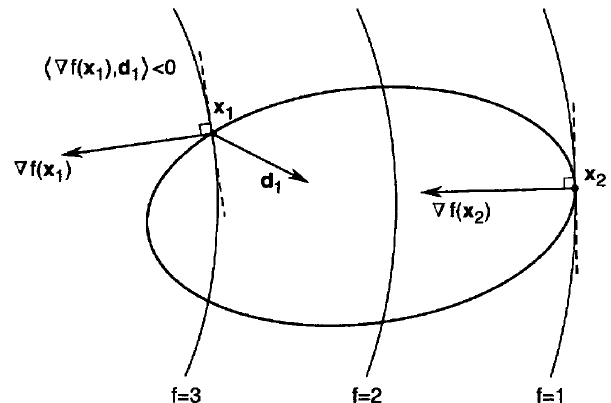
\includegraphics[scale= 0.5]{fonc}
	\centering
    \caption{Γεωμετρική Ερμηνεία της αναγκαίας συνθήκης πρώτης τάξεως FONC.  \cite{chong2013introduction}.}
\end{figure}

Στο παραπάνω σχήμα η $x_1$ δεν ικανοποιεί την ανισότητα \ref{FONC} (συνθήκη FONC) ενώ η $x_2$ την ικανοποιεί. Αυτό συμβαίνει γιατί στο σημείο $x_1$ το εσωτερικό γινόμενο $\langle \nabla f(x_1),\textbf{d}_1\rangle$ ισούται με $||\nabla f(x_1)|| \cdot ||\textbf{d}_1|| cos(\theta_1)$. Αλλά είναι εμφανές στο σχήμα πως το συνημίτονο της γωνίας μεταξύ του $\nabla f(x_1)$ και του διανύσματος κατεύθυνσης $\textbf{d}_1$ είναι αρνητικό. Και αυτό γιατί η γωνία είναι μεγαλύτερη από $90^о$.

Στην περίπτωση του $x_2$ η γωνία μεταξύ του $\nabla f(x_2)$ και του διανύσματος κατεύθυνσης $\textbf{d}_2$ είναι $90^ο$ και οπότε το συνημίτονό της μηδενίζεται. Άρα η συνθήκη FONC (\ref{FONC}) ικανοποιείται.

\begin{thm}{\textbf{Αναγκαία Συνθήκη Δεύτερης Τάξης (SONC).}}
	Έστω A υποσύνολο του $\mathbb{R}^n$, μια συνάρτηση $f\in C^2$ στο Α, $x^*$ ένα τοπικό ελάχιστο της $f$ στο Α και $d$ η κατεύθυνση στο $x^*$. Εάν $d^T\nabla f(x^*)=0$, τότε :
	\begin{align}
		d^TH(x^*)d \geq 0
	\end{align}
\end{thm}

Ακολουθεί ένα παράδειγμα όπου βλέπουμε πώς μπορούν να αξιοποιηθούν οι παραπάνω συνθήκες  FONC, SONC.

\begin{exmp}
	Έστω η συνάρτηση $f:\mathbb{R}^2\rightarrow \mathbb{R}$ με $f(x_1,x_2) = x_1^2-x_2^2$. Θα εξετάσουμε ποιες από τις δύο προηγούμενες συνθήκες ($FONC, SONC$) ικανοποιούνται.
\end{exmp}
\textbf{Λύση}

Βρίσκουμε αρχικά ότι $\nabla f(x_1,x_2) = \begin{pmatrix}
2x_1\\
-2x_2
\end{pmatrix}$
Η συνθήκη FONC απαιτεί να ισχύει $\nabla f(x)=0$ . Έτσι στη συγκεκριμένη περίπτωση θα πρέπει $x=\begin{pmatrix}
x_1\\
x_2
\end{pmatrix} = \begin{pmatrix}
0\\
0
\end{pmatrix}$
Σχετικά με τη δεύτερη συνθήκη SONC αρχικά υπολογίζουμε τον εσσιανό πίνακα, Έτσι βρίσκουμε :\begin{align*}
H(x) = \begin{pmatrix}
2 & 0\\
0 & -2
\end{pmatrix}
\end{align*}
Παρατηρούμε ότι ο Εσσιανός έιναι αόριστος επομένως για κάποια $d_1, d_2 \in \mathbb{R}^2$ θα ισχύουν:
\begin{align*}
d_1^TH(x)d_1 > 0 \hspace{0.3cm} \text{και} \hspace{0.3cm} d_2^TH(x)d_2 < 0
\end{align*}
Για παράδειγμα έστω τα $d_1 = \begin{pmatrix}
1\\ 0
\end{pmatrix}$
και $d_2 = \begin{pmatrix}
0\\ 1
\end{pmatrix}$
Επομένως το σημείο $x=\begin{pmatrix}
x_1\\
x_2
\end{pmatrix} = \begin{pmatrix}
0\\
0
\end{pmatrix}$ ικανοποιεί την συνθήκη FONC αλλά όχι τη συνθήκη SONC, άρα δεν αποτελεί ελάχιστο για τη συνάρτηση f. Μια γεωμετρική εικόνα παίρνουμε και από το ακόλουθο γράφημα :
\begin{figure}[H]	
	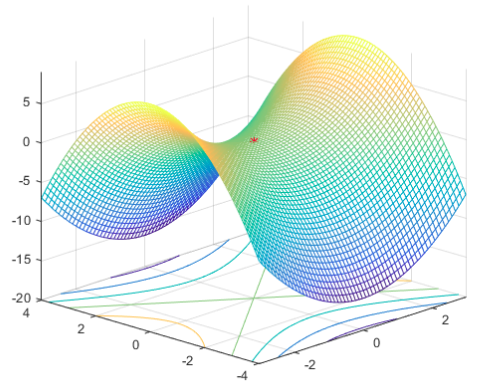
\includegraphics[scale= 0.5]{fonc-sonc}
	\centering
    \caption{To γράφημα της συνάρτησης $f(x_1,x_2) = x_1^2-x_2^2$. Το σημείο $(0,0)^T$ ικανοποιεί τη FONC αλλά όχι τη SONC.}
\end{figure}
Λόγω του παραπάνω προβλήματος διατυπώνουμε την επαρκή συνθήκη δεύτερης τάξης όπως δίνεται από το επόμενο θεώρημα.

\begin{thm}{\textbf{Επαρκής Συνθήκη δεύτερης τάξης (SOSC).}}
Έστω μια συνάρτηση $f\in C^2$ ορισμένη σε μια περιοχή όπου το $x^*$ είναι εσωτερικό σημείο. 

Έστω ακόμα ότι :

\begin{enumerate}
	\item $\nabla f(x^*) = 0 $
	\item $H(x^*) = 0$
\end{enumerate}

Τότε το $x^*$ είναι \textbf{αυστηρά} τοπικό ελάχιστο της $f$	
\end{thm}

%\newpage
\section{Μέθοδοι μονοδιάστατης βελτιστοποίησης}
\subsubsection{Μονοδιάστατη μέθοδος Newton}
Η μέθοδος Newton \footnote{\url{https://en.wikipedia.org/wiki/Newton's\_method}} ή καλύτερα η μέθοδος των Newton-Raphson είναι η πιο "δημοφιλής" μέθοδος για τη λύση μη γραμμικών εξισώσεων, διότι είναι απλή στην εφαρμογή της και επί πλέον, για απλές ρίζες είναι τετραγωνικής σύγκλισης (άρα αρκετά γρήγορη σε σχέση με άλλες μεθόδους).

Ξεκινάει από ένα τυχαίο σημείο του πεδίου ορισμού που καλό είναι να βρίσκεται πλησίον της ρίζας και δίνεται από τον επαναληπτικό τύπο :
\begin{equation}
x^{(k+1)} = x^{(k)} - \frac{f(x^{(k)})}{f'(x^{(k)})}
\end{equation}
όπου k αντιστοιχεί στον αριθμό της εκάστοτε επανάληψης.

\begin{figure}[H]
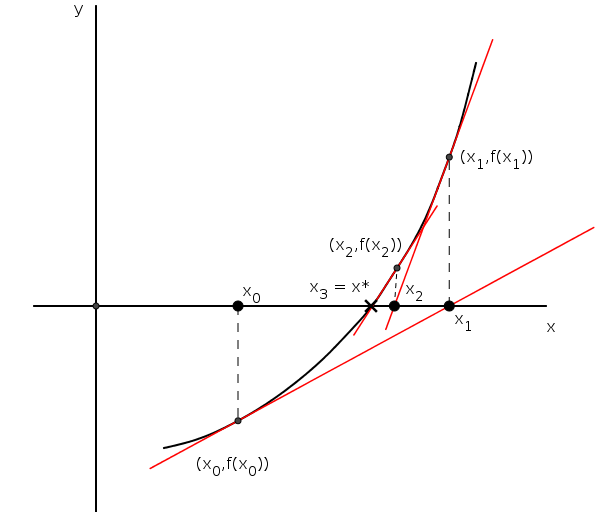
\includegraphics[scale=0.5]{Newton1}
\centering
    \caption{Γεωμετρική Ερμηνεία της μονοδιάστατης μεθόδου Newton}
\end{figure}

%\underline{\textbf{Τετραγωνική σύγκλιση της μεθόδου}}\\
\subsubsection{Τετραγωνική σύγκλιση της μεθόδου}

Έστω ότι η συνάρτηση $f$ είναι δύο φορές συνεχώς παραγωγίσιμη. Από τη μέθοδο Newton ισχύει :
\begin{align*}
x^{(k+1)} = x^{(k)} - \frac{f(x^{(k)})}{f'(x^{(k)})}
\end{align*}
Αν $x^*$ είναι η ρίζα της f τότε από τη μέθοδο Newton πρυκύπτει :
\begin{align*}
g(x) = x - \frac{f(x)}{f'(x)} \hspace{0.2cm} \text{και} \hspace{0.2cm} g(x^*)=x^*, \hspace{0.2cm} g'(x) = \frac{f(x)f'(x)}{[f'(x)]^2}
\end{align*}

Για να προσεγγίσουμε τη συνάρτηση g θα χρησιμοποιήσουμε ένα πεπερασμένο πλήθος όρων της σειράς Taylor\footnote{\url{https://en.wikipedia.org/wiki/Taylor\_series}}.

Αναπτύσουμε τη $g(x)$ κατά Taylor κοντά στη ρίζα $x^*$. Άρα :
\begin{align*}
g(x) = g(x^*) + (x-x^*)g'(x^*) + (x-x^*)^2\frac{g''(\xi)}{2!}, \hspace{0.2cm} \xi \in (x,x^*)
\end{align*}
Είδαμε ότι $g(x^*)=x^*$ και επιπλέον παρατηρούμε ότι : $g'(x^*)=0$ ενώ $g''(x^*)\neq 0$.
Συνεπώς :
\begin{align*}
\begin{split}
g(x) &= x^* + \frac{1}{2}(x-x^*)^2g''(\xi)\\
g(x) - x^* &= \frac{1}{2}(x-x^*)^2g''(\xi)\\
x^{(k+1)} - x^* &= \frac{1}{2}(x^{(k)}-x^*)^2g''(\xi)\\
|\varepsilon ^{(k+1)}| &\leq c\cdot|\varepsilon^k|^2
\end{split}
\end{align*}
Άρα η σύγκλιση είναι τετραγωνική αφού το σφάλμα στη νέα επανάληψη είναι ανάλογο του τετραγώνου του σφάλματος της προηγούμενης.

\subsubsection{Μέθοδος της τέμνουσας (Secant Method)}

Η μέθοδος Newton με χρήση παραγώγων 2ης τάξης παίρνει τη μορφή :
\begin{align*}
x^{(k+1)} = x^{(k)} - \frac{f'(x^{(k)})}{f''(x^{(k)})}
\end{align*}
Σε περίπτωση όπου δεν είναι δυνατός ο υπολογισμός της 2ης παραγώγου, τότε δοκιμάζουμε να την προσεγγίσουμε μέσω της παραγώγου πρώτης τάξης. Δηλαδή προσεγγίζουμε την $f''(x^{(k)})$ μέσω του τύπου :
\begin{align*}
\frac{f'(x^{(k)})-f'(x^{(k-1)})}{x^{(k)}-x^{(k-1)}}
\end{align*}
Έτσι μέσω της παραπάνω προσέγγισης λαμβάνουμε τον επαναληπτικό τύπο της μεθόδου της τέμνουσας :
\begin{align*}
\begin{split}
x^{(k+1)} &= x^{(k)} - \frac{x^{(k)}-x^{(k-1)}}{f'(x^{(k)})-f'(x^{(k-1)})}f'(x^{(k)})\\
x^{(k+1)} &= \frac{f'(x^{(k)})x^{(k-1)}-f'(x^{(k-1)})x^{(k)}}{f'(x^{k})-f'(x^{k-1})}
\end{split}
\end{align*}
Παρατηρούμε ότι η μέθοδος της τέμνουσας απαιτεί δύο αρχικά σημεία για να ξεκινήσει, έστω τα $x^{(-1)}$ και $x^{(0)}$. Όπως και στη μέθοδο Newton, έτσι και στη μέθοδο της τέμνουσας δεν συμπεριλαμβάνεται τιμές της $f(x^{(k)})$, αντίθετα προσπαθούμε να μηδενίσουμε την παράγωγο.

\begin{figure}[H]
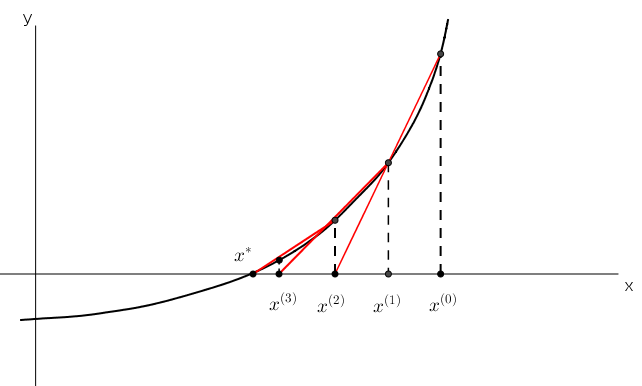
\includegraphics[scale=0.5]{secant}
\centering
    \caption{Γεωμετρική Ερμηνεία της μεθόδου της τέμνουσας}
\end{figure}
     %%%Από αυτό το κεφάλαιο θα'λεγα να αναφέρουμε κυρίως την μέθοδο του Νεύτωνα και της τέμνουσας. Αν έχουμε όρεξη συζητάμε και αυτήν της Χρυσής τομής (ή του Fibonnaci).


%%%%%%%%%%%%%%%%%%%%%%%%%%%%%%%%%%%%%%%%%%%%%%%%%%%%%%%%%%%%%%%%%%%%%%%%%%%%%%%%%%%%%
%%%%%%% 		Capitulo 3 |  principais avancos em relacao ao ultimo relatorio %%%%%
%d. Situação do projeto de pesquisa à época do último relatório;
%–no mínimo 1 (uma) e no máximo 2 (duas) páginas–;
%%%%%%%%%%%%%%%%%%%%%%%%%%%%%%%%%%%%%%%%%%%%%%%%%%%%%%%%%%%%%%%%%%%%%%%%%%%%%%%%%%%%%
\newpage
\chapter{Μέθοδοι Πολυδιάστατης Βελτιστοποίησης Χωρίς Περιορισμούς}

\section{Μέθοδοι Κλίσης}
\subsection{Εισαγωγικά για τις μεθόδους κλίσης}
    Το gradient της f στο $x_{0}$, $\nabla f(x_{0})$ εάν δεν είναι 0 τότε είναι κάθετο στο διάνυσμα της εφαπτομένης στο σημείο αυτό. Έτσι το gradient κινείται στην κατεύθυνση εκείνη τέτοια ώστε η συνάρτηση να μεγιστοποιεί την άυξηση ή τη μείωση στην κατεύθυνση του gradient παρά σε οποιαδήποτε άλλη κατεύθυνση. 
    
\begin{figure}[H]
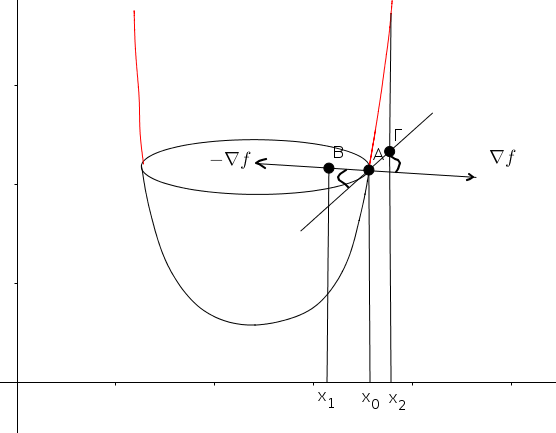
\includegraphics[scale=0.5]{3}
\centering
    \caption{Γράφημα κατέυθυνσης των $\nabla f(x)$ και $-\nabla f(x)$}
\end{figure}

%%%%%% ΠΡΟΣΘΕΣΕ ΑΝΙΣΟΤΗΤΑ ΚΩΣΥ ΣΒΑΡΤΖ
Για τα επόμενα θα χρειαστούμε το ακόλουθο σημαντικό θεώρημα από την γραμμική άλγεβρα, οπότε το διατυπώνουμε ακολούθως:

\begin{thm}[Ανισότητα Cauchy-Schwarz] Για κάθε διάνυσμα \textbf{x,y} $\in \mathbb{R}^n$ ισχύει η ανισότητα:

\begin{equation}\label{cauchy-ineq}
	|\langle \textbf{x,y}\rangle| \leq ||\textbf{x}||||\textbf{y}||
\end{equation}

Επίσης, η ισότητα ισχύει αν και μόνο αν το \textbf{x} είναι γραμμικός συνδυασμός του \textbf{y}, δηλαδή αν $\textbf{x} = \alpha \textbf{y}$, για κάποιο $\alpha\in \mathbb{R}$.
\end{thm}

Από την ανισότητα \textbf{Cauchy-Schwarz} (\ref{cauchy-ineq}) παίρνουμε: 
\begin{align*}
\langle\nabla f(x), \textbf{d}\rangle = ||\nabla f(x)||\cdot||\textbf{d}||  \leq ||\nabla f(x)||, \hspace{0.2cm} \text{για  } ||\textbf{d}||=1
\end{align*}

Δηλαδή για κάθε κατεύθυνση \textbf{d} με μοναδιαίο μέτρο, ο ρυθμός της μέγιστης αύξησης της f στο x, $\langle\nabla f(x), \textbf{d}\rangle$ έχει μέγιστη τιμή $||\nabla f(x)||$.

Οπότε αν θέσουμε ως κατεύθυνση $\textbf{d} = \nabla f(x)/||\nabla f(x)||$ παίρνουμε:
\begin{align*}
\langle\nabla f(x), \frac{\nabla f(x)}{||\nabla f(x)||}\rangle = ||\nabla f(x)||\cdot||\textbf{d}||= ||\nabla f(x)||
\end{align*}
Επομένως από τα παραπάνω καταλήγουμε ότι η κατεύθυνση στην οποία δείχνει η κλίση της $f(x)$, $\nabla f(x)$, είναι η \textbf{κατεύθυνση μέγιστης αύξησης} της f	στο x. Άρα η κατεύθυνση του $-\nabla f(x)$ είναι η \textbf{κατεύθυνση μέγιστης μείωσης} της f και η οποία έιναι η πλέον κατάλληλη για αναζήτηση των global minimizers.

Στη συνέχεια αν θεωρήσουμε ένα αρχικό σημείο $x_0$ τότε ο προηγούμενος τύπος των Line search μεθόδων: 
\begin{align*}
x^{(k+1)} = x^{(k)} + a^{(k)}d^{(k)}
\end{align*}
για την πρώτη επανάληψη  και για $d^{(k)} = -\nabla f(x_k)$ θα γίνει : 
\begin{align*}
x^{(1)} = x^{(0)} - a^{(0)}\nabla f(x^{(0)})
\end{align*}
Έτσι μέσω του αλγορίθμου αυτού καταλήγουμε στον τύπο : $x^{(k+1)} = x^{(k)} - a^{(k)}\nabla f(x^{(k)})$\\
Γενικότερα αναφερόμαστε στον παραπάνω τύπο ως ο \textbf{αλγόριθμος gradient descent}.

\begin{rem}
Αν συνεχίσουμε την παραπάνω διαδικασία της πρώτης επανάληψης\\ $x_1 = x_0 - a_0\nabla f(x_0)$, τότε από το Θεώρημα Taylor \footnote{\url{https://en.wikipedia.org/wiki/Taylor\%27s\_theorem}} παίρνουμε :
\begin{align*}
f(x^{(0)} - a^{(0)}\nabla f(x^{(0)})) = f(x^{(0)}) - a^{(0)}||\nabla f(x^{(0)})|| + o(a) 
\end{align*}
έτσι για $\nabla f(x_0) \neq 0$ και σχετικά μικρό βήμα α, παίρνουμε : 
\begin{align*}
f(x^{(0)} - a^{(0)}\nabla f(x^{(0)})) < f(x^{(0)})
\end{align*}
Επομένως το $x^{(0)} - a^{(0)}\nabla f(x^{(0)})$ αποτελεί βελτίωση του $x_0$ αν ψάχνουμε για ολικό ελαχιστοποιητή.
\end{rem}

%\underline{\textbf{\large{Ισο{\"υ}ψείς}}}\\
%\subsection{Ισο{\"υ}ψείς}
\subsection{Ισοϋψείς Καμπύλες}
Πρώτα απ' όλα να σημειωθεί ότι στο χώρο η συναρτησιακή τιμή είναι ένα επίπεδο που "κόβει" την καμπύλη και είναι παράλληλο με το $z=0$. Ακουλουθεί και ενδεικτικό σχήμα:
\begin{figure}[H]
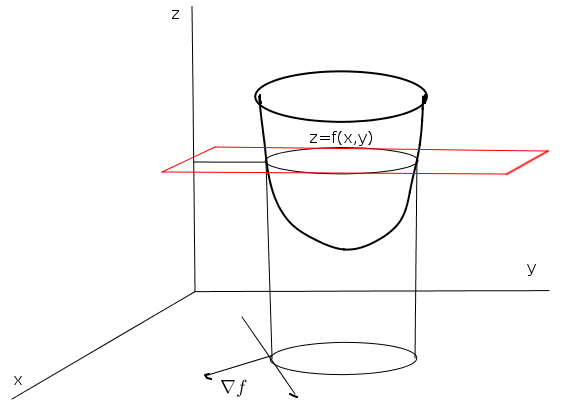
\includegraphics[scale=0.5]{4}
\centering
    \caption{Απεικόνιση της συναρτησιακής τιμής στο χώρο}
\end{figure}

\begin{defn}
Ισοϋψής καμπύλη καλείται ο γεωμετρικός τόπος των σημείων που έχουν την ίδια συναρτησιακή τιμή. Δηλαδή σε μαθηματική μορφή μια ισοϋψής καμπύλη είναι το σύνολο $C_1 = \{\forall x \forall y| f(x,y) = c\}.$
\end{defn}

Στο παρακάτω σχήμα βλέπουμε ουσιαστικά τρεις συναρτησιακές τιμές οι οποίες απεικονίζονται στο χώρο αλλά και στο επίπεδο. Αν παρατηρήσουμε τις καμπύλες στο επίπεδο, τότε καθώς κινούμαστε προς το εσωτερικό δηλαδη τη μικρότερη (ως προς το εμβαδό) καμπύλη, κατευθυνόμαστε σε μικρότερη συναρτησιακή τιμή. Άρα ακολουθούμε την κατεύθυνση του $-\nabla f(x,y)$.

\begin{figure}[H]
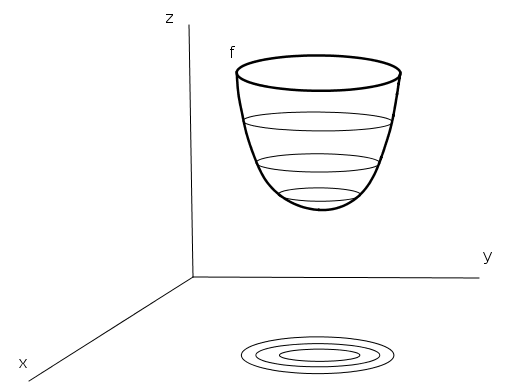
\includegraphics[scale=0.5]{5}
\centering
    \caption{Aπεικόνιση στο χώρο και το επίπεδο $xy$}
\end{figure}

Εάν μεγενθύνουμε κατάλληλα το προηγούμενο σχήμα και συγκεριμένα στο επίπεδο που απεικονίζονται οι τρεις καμπύλες τότε θα είχαμε μια εικόνα σαν την παρακάτω

\begin{figure}[H]
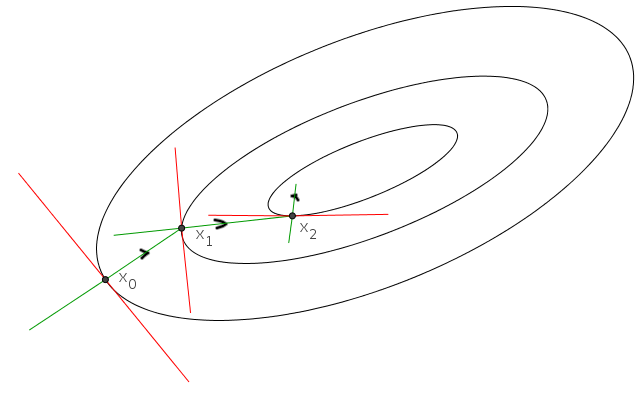
\includegraphics[scale=0.5]{6}
\centering
\end{figure}

Στο παραπάνω σχήμα παρατηρούμε τα ακόλουθα άξια αναφοράς:

\begin{itemize}
\item Οι κόκκινες γραμμές αντιστοιχούν στις εφαπτομένες της εκάστοτε καμπύλης στα σημεία $x_0, x_1$ και $x_2$ καθώς κινούμαστε σε μικρότερη καμπύλη αντίστοιχα.
\item Οι πράσινες γραμμές αντιστοιχούν στις κατευθύνσεις των $\nabla f$ (από μικρότερες προς μεγαλύτερες καμπύλες) και $-\nabla f$ (από μεγαλύτερες προς μικρότερες καμπύλες), γι' αυτό και έχουν διεύθυνση κάθετη στις εφαπτομένες.
\end{itemize}
%\hspace{-0.7cm}
\underline{\textbf{Συμπέρασμα :}} Βλέπουμε ότι καθώς κινούμαστε σε μικρότερη καμπύλη, δηλαδή από το $x_0$ στο $x_1$ και από αυτό στο $x_2$ μειώνεται αντίστοιχα και η συναρτησιακή τιμή, όπως φαίνεται καλύτερα και στο παραπάνω σχήμα.

\subsection{Μέθοδος Απότομης Καθόδου (Steepest Descent)}
Η μέθοδος Steepest Descent αποτελεί έναν αλγόριθμος κλίσης όπου το βήμα $a_{k}$ επιλέγεται κατάλληλα ώστε να έχουμε τη μέγιστη δυνατή μείωση της συναρτησιακής τιμής. Δηλαδή το βήμα επιλέγεται τ.ω. να ελαχιστοποιείται η συνάρτηση :
\begin{align*}
\phi(a) = f(x^{(k)} - a\nabla f(x^{(k)}))
\end{align*}
Tελικά σε αυτή τη μέθοδο σε κάθε βήμα ξεκινώντας από ένα αρχικό σημείο (διάνυσμα για μεγαλύτερες διαστάσεις) \textbf{x}$^{(0)}$ γίνεται ένα  βήμα line search στην κατεύθυνση του $-\nabla f(x^{(k)})$ μέχρι την εύρεση του ζητούμενου ελαχιστοποιητή $x^{(k+1)}$. Ακολουθεί και ενδεικτικό σχήμα :
\begin{figure}[H]
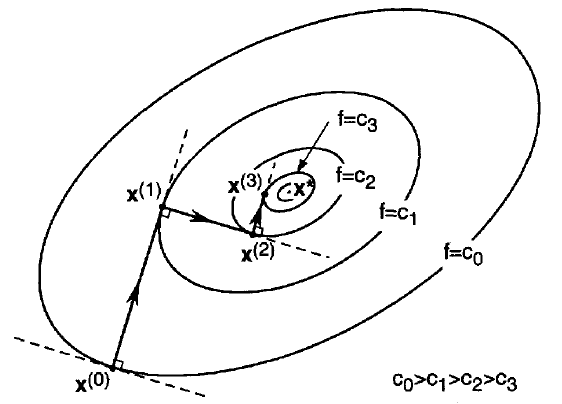
\includegraphics[scale=0.5]{steepest}
\centering
\end{figure}


\begin{thm}
Εάν $\{ x^{(k)}\}_{k=0}^{\infty}$ είναι μια ακολουθία απότομης καθόδου για μια συνάρτηση $f:\mathbb{R} ^n \rightarrow \mathbb{R}$, τότε για κάθε k το διάνυσμα $x^{(k+1)} - x^{(k)}$ θα είναι ορθογώνιο ως προς το διάνυσμα $x^{(k+2)} - x^{(k+1)}$.
\end{thm}

\textbf{Απόδειξη:}\\
Από τον επαναληπτικό τύπο για τη μέθοδο steepest descent προκύπτει άμεσα ότι :
\begin{align*}
\langle x^{(k+1)} - x^{(k)}, x^{(k+2)} - x^{(k+1)}\rangle = a^{(k)}a^{(k+1)}\langle\nabla f(x^{(k)}), \nabla f(x^{(k+1)})\rangle
\end{align*}
Επομένως αρκεί να δείξουμε ότι $\langle\nabla f(x^{(k)}), \nabla f(x^{(k+1)})\rangle=0$

To βήμα $a^{(k)}$ είναι τέτοιο ώστε να ελαχιστοποιεί τη συνάρτηση
\begin{align*}
\phi_k(a) = f(x^{(k)} - a^k\nabla f(x^{(k)}))
\end{align*}
Έτσι με χρήση της συνθήκης \textbf{FONC} θα πάρουμε :
\begin{equation}
\begin{split}
0 &= \phi _k '(a^{(k)}) \\
&= \frac{d\phi _k}{da}(a^{(k)}) \\
&= \nabla f(x^{(k)} - a^{(k)}\nabla f(x^{(k)}))^T(-\nabla f(x^{(k)})) \\
&= - \langle\nabla f(x^{(k+1)}),\nabla f(x^{(k)})\rangle
\end{split}
\end{equation}

Από το παραπάνω θεώρημα προκύπτει το ακόλουθο πόρισμα. 

\begin{cor}
Εάν $\{ x^{(k)}\}_{k=0}^{\infty}$ είναι μια  ακολουθία steepest descent για μια συνάρτηση \\$f:\mathbb{R} ^n \rightarrow \mathbb{R}$ και $\nabla f(x^{(k)}) \neq 0$ τότε $f(x^{(k+1)})<f(x^{(k)})$.
\end{cor}

Τα κριτήρια τερματισμού μιας ακολουθίας απότομης καθόδου είναι:

%\newpage
%\underline{\textbf{Κρίτήρια τερματισμού}}
\subsubsection{Κριτήρια τερματισμού}
\begin{itemize}
\item $\nabla f(x^{(k+1)}) = 0$
\vspace{-0.2cm}
\item $|f(x^{(k+1)}) - f(x^{(k)})| < \varepsilon$, όπου $\varepsilon >0$
\vspace{-0.2cm}
\item $||x^{(k+1)} - x^{(k)}||<\varepsilon$
\vspace{-0.2cm}
\item $\frac{|f(x^{(k+1)}) - f(x^{(k)})|}{|f(x^{(k)})|}<\varepsilon$
\vspace{-0.2cm}
\item $\frac{||x^{(k+1)} - x^{(k)}||}{||x^{(k)}||} < \varepsilon$
\end{itemize}

%\underline{\textbf{Συμπεριφροά της steepest descent για τετραγωνικές συναρτήσεις}}\\
\subsubsection{Συμπεριφορά της steepest descent για τετραγωνικές συναρτήσεις}

Έστω η συνάρτηση της μορφής $f(x) = \frac{1}{2}x^TQx-b^Tx$, όπου $Q\in \mathbb{R}^{n\times n}$ είναι ένας θετικά ορισμένος πίνακας, $b\in \mathbb{R}^{n}$ και $x\in \mathbb{R}^{n}$. Το ολικό ελάχιστο της f μπορεί να βρεθεί θέτοντας το gradient της f ίσο με το μηδέν. Δηλαδή :
\begin{align*}
\nabla f(x) = Qx-b = 0
\end{align*}
Ο εσσιανός πίνακας της f είναι ο $H(x)=Q=Q^T>0$. Επομένως ο αλγόριθμος steepest descent για μια τετραγωνική συνάρτηση της παραπάνω μορφής θα δίνεται από το ακόλουθο επαναληπτικό σχήμα.
\begin{align}
x^{(k+1)} = x^{(k)} - a^{k}\nabla f(x^{(k)})
\end{align}

Έστω τώρα ότι $\nabla f(x^{(k)})\neq 0$. Εφαρμόζοντας τη συνθήκη \textbf{FONC} στη συνάρτηση $\phi_k(a) = f(x^{(k)} - a^k\nabla f(x^{(k)}))$ θα πάρουμε 
\begin{align*}
\phi' _k(a) = (x^{(k)} - a^k\nabla f(x^{(k)}))^T(-\nabla f(x^{(k)})) - b^T(-\nabla f(x^{(k)}))
\end{align*}
Επομένως $\phi' _k(a) = 0$ αν $(x^{(k)} - a^k\nabla f(x^{(k)}))^T(-\nabla f(x^{(k)})) = b^T(-\nabla f(x^{(k)}))$
Τελικά καταλήγουμε για το βήμα ότι δίνεται από τον τύπο :
\begin{align*}
a^{(k)} = \frac{\nabla f(x^{(k)})^T\nabla f(x^{(k)})}{\nabla f(x^{(k)})^TQ\nabla f(x^{(k)})}
\end{align*}
% Μέθοδος πολυδιάστατης Newton------------------------------------------------------
\section{Μέθοδος πολυδιάστατης Newton}

%% Μέθοδοι Quasi Newton
\section{Μέθοδοι Quasi Newton}
Γύρω στο 1950, ένας φυσικός ονόματι W.C. Davidon, εργαζότανε πάνω σε μεγάλα προβλήματα υπολογισμών βελτιστοποίησης στο Argonne National Laboratory χρησιμοποιώντας τη μέθοδο $coordinate-descent$. Ο αλγόριθμος τον οποίο ανέπτυξε ήταν ο πρώτος $Quasi-Newton$ αλγόριθμος. Γρήγορα αποδείχθηκε από τους Fletcher και Powell, ότι ο νέος αυτός αλγόριθμος ήταν πιο γρήγορος και πιο αξιόπιστος από οποιοδήποτε άλλη μέθοδο που υπήρχε εκείνη τη στιγμή.

Οι μέθοδοι Quasi-Newton όπως και οι μέθοδοι steepest descent, απαιτούν μόνο τον υπολογισμό του gradient της αντικειμενικής συνάρτησης σε κάθε επανάληψη. Ελέγχοντας τις αλλαγές του gradient σε κάθε επανάληψη κατασκευάζουν ένα μοντέλο της συνάρτησης που είναι αρκετά καλό για "υπεργραμμική" σύγκλιση. Η βελτίωση σε σχέση με τις μεθόδους Steepest descent είναι δραματική, ειδικά σε δύσκολα προβλήματα. Τέλος δεν απαιτείται ο υπολογισμός παραγώγων δεύτερης τάξης και για αυτό το λόγο αρκετές φορές οι Quasi Newton μέθοδοι είναι πιο αποτελεσματικοί από τη μέθοδο Newton\cite{nocedal2006numerical}.


\subsection{BFGS \& DFP}
H πιο γνωστή Quasi-Newton μέθδος είναι η \textbf{BFGS} η οποία πήρε το όνομα της από τους δημιουργούς της, Broyden, Fletcher, Goldfarb, και Shanno. Έστω ότι το μοντέλο της αντικειμενικής συνάρτησης στην τρέχουσα επανάληψη $x^{(k)}$ είναι :
\begin{align}
m^{(k)}(d) = f_k + \nabla f_k^Td+\frac{1}{2}d^TB_kd
\end{align}
και ο επαναληπτικός τύπος  δίνεται αρχικά ως εξής :
\begin{align}
x^{(k+1)} = x^{(k)} + a^{(k)}d^{(k)}
\end{align}
όπου $a^{(k)}$ είναι το κατάλληλο βήμα που ικανοποιεί τις συνθήκες Wolfe\footnote{\url{https://en.wikipedia.org/wiki/Wolfe\_conditions}} και συγκεκριμένα η συνθήκη $f(x^{(k+1)}) < f(x^{(k)})$. 

Επιπλέον η κατεύθυνση $d^{(k)}$ είναι κατεύθυνση μείωσης και δίνεται από τον τύπο :
\begin{align}
d^{(k)} = -B_k^{-1}\nabla f_k
\end{align}
και $B_k$ είναι ένας θετικά ορισμένος πίνακας που αποτελεί προσέγγιση του Εσσιανού πίνακα $H_k$.

Αντί του υπολογισμού του $B_k$ σε κάθε επανάληψη, ο Davidon πρότεινε την ανανέωση του πίνακα λαμβάνοντας υπόψιν την καμπυλότητα όπως αυτή έχει μετρηθεί στο πιο πρόσφατο βήμα. Έστω ότι έχουμε κατασκευάσει τη νέα επανάληψη $x^{(k+1)}$ και θέλουμε να κατασκευάσουμε ένα νέο μοντέλο με τετραγωνική λειτουργία :
\begin{align}
m^{(k+1)}(d) = f_{k+1} + \nabla f_{k+1}^Td + \frac{1}{2} d^TB_{k+1}d
\end{align}
Mια βασική απαίτηση είναι ότι το gradient του νέου μοντέλου θα πρέπει να ταυτίζεται με το gradient της αντικειμενικής συνάρτησης στις 2 τελευταίες επαναλήψεις $x^{(k)}$ και $x^{(k+1)}$. Έτσι θα έχουμε 
\begin{align}
\nabla m^{(k+1)}(-a^{(k)}d^{(k)}) = \nabla f_{k+1} - a^{(k)}B_{k+1}d^{(k)} = \nabla f_k
\end{align}
ή ισοδύναμα 
\begin{align}\label{eq1}
B_{k+1}a^{(k)}d^{(k)} = \nabla f_{k+1} - \nabla f_{k}
\end{align}
Εάν ορίσουμε τα διανύσματα 
\begin{align}
s^{(k)} = x^{(k+1)} - x^{(k)} \hspace{0.1cm} \text{και} \hspace{0.1cm} y_k = \nabla f_{k+1} - \nabla f_{k}
\end{align}
τότε η \ref{eq1} γίνεται 
\begin{align}\label{eq2}
B_{k+1}s^{(k)} = y_k
\end{align}
στην οποία αναφερόμαστε ως εξίσωση τέμνουσας ($secant$ $equation$).

H εξίσωση της τέμνουσας (secant) απαιτεί ο θετικά ορισμένος πίνακας $B_{k+1}$ να απεικονίζει το $s^{(k)}$ στο $y_k$. Για να ισχύει αυτό θα πρέπει να ικανοποιείται η συνθήκη καμπυλότητας 
\begin{align}
s^{(k)T}y_k > 0
\end{align}
όταν η συνθήκη αυτή ικανοποιείται, η εξίσωση \ref{eq2} έχει πάντα μια λύση $B_{k+1}$.

Για να καθορίσουμε πλήρως το $B_{k+1}$ εισάγουμε τη συνθήκη που λέει "μεταξύ όλων των συμμετρικών πινάκων που ικανοποιούν την εξίσωση της τενουσας, ο $B_{k+1}$ είναι ο πιο κοντινός του $B_{k}$." Δηλαδή επιλύουμε το πρόβλημα :
\begin{align}\label{eq3}
\min_{B}||B-B_k||\\
B=B^T, \hspace{0.1cm} Bs^{k} = y_k
\end{align}
όπου τα $s^{k}, y_k$ ικανοποιούν τη συνθήκη καμπυλότητας και ο $B_k$ είναι συμμετρικός και θετικά ορισμένος. Στη σχέση \ref{eq3} μπορούν να χρησιμοποιούν πολλές νόρμες αλλά εμείς θα προτιμήσουμε τη σταθμισμένη νόρμα Frobenius\footnote{\url{https://en.wikipedia.org/wiki/Low-rank\_approximation\#Weighted\_low-rank\_approximation\_problems}} που ορίζεται ως εξής :
\begin{align*}
||A||_W \equiv ||W^{\frac{1}{2}}AW^{\frac{1}{2}}||_F\\
||C||^2_F = \sum_{i=1}^{n}\sum_{j=1}^{n}c^2_{ij}
\end{align*}
Το βάρος W επιλέγεται ως ο πίνακας που ικανοποιεί τη σχέση $Wy_k = s^{(k)}$.

Συγκεκριμένα, μπορούμε να επιλέξουμε ως πίνακα-βάρος τον $W = \overline{G}_k^{-1}$ όπου με $\overline{G}_k$ ορίζεται \cite{nocedal2006numerical} η μέση τιμή του εσσιανού πίνακα:
\begin{align}
\overline{G}_k = [\int_0^1 \nabla ^2f(x^{(k)} + \tau a^{(k)}d^{(k)}) d\tau]\\
y_k = \overline{G}_ka^{(k)}d^{(k)} = \overline{G}_ks^{(k)}
\end{align}
Με τον σταθμισμένο πίνακα και την παραπάνω νόρμα η λύση της \ref{eq3} είναι
\begin{align}\label{leq}
B_{k+1} = (I - \gamma_ky_ks^{(k)T})B_k(I - \gamma_ks^{(k)}y_k ^T) + \gamma_ky_ky_k ^T \hspace{0.25cm} (\textbf{DFP})
\end{align}
 όπου
 \begin{align}
 \gamma_k = \frac{1}{y_k ^Ts^{(k)}}
 \end{align}
 
 O τύπος \ref{leq} καλείται \textbf{τύπος ανανέωσης DFP} (DFP updating formula) από τα ονόματα των Davidon, Fletcher και Powell. Aν θεωρήσουμε τον αντίστροφο του πίνακα $B_k$ ως $H_k = B_k^{-1}$ τότε παίρνουμε τον τύπο 
\begin{align}
H_{k+1} = H_k - \frac{H_ky_ky_k ^TH_k}{y_k ^TH_ky_k} + \frac{s^{(k)}s^{(k)T}}{y_k^Ts^{(k)}} 
\end{align}
Όπως πριν έτσι και τώρα θέλουμε να ισχύουν κάποιες συνθήκες για τον $H_{k+1}$. Οπότε η μοναδική λύση του πίνακα αυτού θα δίνεται από τον τύπο
\begin{align}\label{eq4}
H_{k+1} = (I - \rho_ks^{(k)}y_k ^T)H_k(I -  \gamma_ky_ks^{(k)T}) + \gamma_ks^{(k)}s^{(k)T} \hspace{0.25cm} (\textbf{BFGS})
\end{align}
όπου
\begin{align}
\rho_k=\frac{1}{y_k^Ts^{(k)}}
\end{align}

        
%% Conjugate Newton Methods    
\section{Μέθοδοι Conjugate Direction}
\subsection{Εισαγωγικά}

Οι μέθοδοι $conjugate$ $direction$  βρίσκονται στο ενδιάμεσο των μεθόδων Newton και Steepest Descent. Κάποιες βασικές ιδιότητες των μεθόδων $conjugate$ $direction$ είναι :
\begin{itemize}
\item Επιλύουν τετραγωνικές συναρτήσεις $n$-μεταβλητών σε $n$-βήματα.
\vspace{-0.2cm}
\item H εφαρμογή τους δεν απαιτεί τη χρήση υπολογισμών εσσιανού πίνακα.
\vspace{-0.2cm}
\item Δεν απαιτούν αντιστροφή πινάκων και δεν απαιτείται χώρος για αποθήκευση ενός $n\times n$ μητρώου.
\end{itemize}

Για μια τετραγωνική συνάρτηση $n$ μεταβλητών $f(x) = \frac{1}{2}x^TQx-x^Tb$ με $x\in \mathbb{R}^n$ και $Q=Q^T>0$, η καλύτερη κατεύθυνση αναζήτησης είναι η κατεύθυνση $Q-conjugate$.

\begin{defn}\label{qcon}
Δύο κατευθύνσεις $d^{(1)}, d^{(2)}$ λέμε ότι είναι \textbf{Q-conjugate} όταν : \begin{align*}
d^{(1)T}Qd^{(2)} = 0
\end{align*}
\end{defn}

\begin{defn}
Έστω Q ένας πραγματικός συμμετρικός $n\times n$ πίνακας. Οι κατευθύνσεις $d^{(0)}, d^{(1)}, ..., d^{(n)}$ είναι \textbf{Q-conjugate} αν για κάθε $i\neq j$, έχουμε :
\begin{align*}
d^{(i)T}Qd^{(j)} = 0
\end{align*}
\end{defn}

\begin{cor}
Έστω Q ένας θετικά ορισμένος και συμμετρικός $n\times n$ πίνακας. Αν οι κατευθύνσεις $d^{(0)}, d^{(1)}, ..., d^{(k)}, k\leq n-1$ είναι μη-μηδενικές και \textbf{Q-conjugate} τότε είναι και γραμμικώς ανεξάρτητες.
\end{cor}

Στη συνέχεια θα παρουσιάσουμε το βασικό αλγόριθμο για μεθόδους Conjugate direction. Έστω η τετραγωνική συνάρτηση 
\begin{align*}
f(\textbf{x}) = \frac{1}{2}\textbf{x}^TQ\textbf{x}-\textbf{x}^Tb, \hspace{0.1cm} Q=Q^T>0
\end{align*}
Επειδή Q>0, η συνάρτηση $f$ θα έχει ολικό ελάχιστο το οποίο μπορεί να βρεθεί μέσω της επίλυσης του συστήματος $Qx = b$

Δοθέντος ενός αρχικού σημείου \textbf{x}$^{(0)}$ και των $d^{(0)}, d^{(1)}, ..., d^{(n-1)}$ Q-conjugate κατευθύνσεων, για $k\geq 0$ ορίζουμε τα ακόλουθα μεγέθη :

\begin{align}
\textbf{g}^{(k)} = \nabla f(x^{(k)}) = \textbf{Q}\textbf{x}^{(k)}-b,\\
\alpha ^{(k)} = -\frac{\textbf{g}^{(k)T}\textbf{d}^{(k)}}{\textbf{d}^{(k)T}\textbf{Q}\textbf{d}^{(k)}},\\
x^{(k+1)} = x^{(k)} + \alpha ^{(k)}\textbf{d}^{(k)}
\end{align}

\begin{thm}
Για κάθε αρχικό σημείο $x^{(0)}$, ο βασικός αλγόριθμος conjugate direction συγκλίνει στη μοναδική λύση του συστήματος \textbf{x}$^{*} = $\textbf{x}$^{(n)}$ σε $n$ βήματα.
\end{thm}

\begin{exmp}
Θα ψάξουμε να βρούμε το ολικό ελάχιστο της συνάρτησης 
\begin{align*}
f(x_1,x_2) = \frac{1}{2}\textbf{x}^{T}\begin{bmatrix}
4 & 2\\
2 & 2
\end{bmatrix}\textbf{x} - \textbf{x}^{T}\begin{bmatrix}
-1\\
1
\end{bmatrix}
\end{align*}
με τη μέθοδο conjugate direction και για αρχικό σημείο \textbf{x}$^{(0)}$ = $(0,0)^T$ και κατευθύνσεις $d^{(0)} = [1,0]^T$ και $d^{(1)} = [-\frac{3}{8},\frac{3}{4}]^T$.

\textbf{Λύση}

Αρχικά βρίσκουμε  : 
\begin{align*}
\textbf{g}^{(0)} = -b = [1,-1]^T
\end{align*}
Επομένως
\begin{align*}
\alpha ^{(0)} = -\frac{\textbf{g}^{(0)T}\textbf{d}^{(0)}}{\textbf{d}^{(0)T}\textbf{Q}\textbf{d}^{(0)}} = - \frac{[1,-1][1,0]^T}{[1,0]\begin{bmatrix}
4 & 2\\
2 & 2
\end{bmatrix}[1, 0]^T} = -\frac{1}{4}
\end{align*}
Έτσι για την πρώτη επανάληψη θα πάρουμε :
\begin{align*}
x^{(1)} = x^{(0)} + a^{(0)}d^{(0)} = \begin{bmatrix}
0\\
0
\end{bmatrix}-\frac{1}{4}\begin{bmatrix}
1\\
0
\end{bmatrix} = \begin{bmatrix}
-\frac{1}{4}\\
0
\end{bmatrix}
\end{align*}

Συνεχίζοντας τη διαδικασία για τη 2η επανάληψη θα πρέπει πρώτα να υπολογίσουμε
\begin{align*}
g^{(1)} = Qx^{(1)} - b = \begin{bmatrix}
4 & 2\\
2 & 2
\end{bmatrix}[-\frac{1}{4}, 0]^T - [-1, 1]^T = [0, -\frac{3}{2}]^T
\end{align*}
και
\begin{align*}
\alpha ^{(1)} = -\frac{\textbf{g}^{(1)T}\textbf{d}^{(1)}}{\textbf{d}^{(1)T}\textbf{Q}\textbf{d}^{(1)}} = -\frac{[0, -\frac{3}{2}][-\frac{3}{8}, \frac{3}{4}]^T}{[-\frac{3}{8}, \frac{3}{4}]\begin{bmatrix}
4 & 2\\
2 & 2
\end{bmatrix}[-\frac{3}{8}, \frac{3}{4}]^T} = 2
\end{align*}
Επομένως :
\begin{align*}
x^{(2)} = x^{(1)} + a^{(1)}d^{(1)} = [-\frac{1}{4}, 0]^T + 2[-\frac{3}{8}, \frac{3}{4}]^T = [-1, \frac{3}{2}]^T
\end{align*}
Τελικά καταλήξαμε στη λύση που είναι η $x^* = x^{(2)}$
\end{exmp}

\begin{cor}
Στον  αλγόριθμο conjugate direction, αποδεικνύεται ότι 
\begin{align*}
\textbf{g}^{(k+1)T}\textbf{d}^{(i)} = 0,\hspace{0.2cm} \forall k, 0\leq k \leq n-1, \hspace{0.1cm}και \hspace{0.1cm} 0\leq i \leq k
\end{align*}
\end{cor}

Από το προηγούμενο πόρισμα προκύπτει ότι το διάνυσμα \textbf{g}$^{(k+1)}$ είναι ορθογώνιο με οποιοδήποτε διάνυσμα από τα $d^{(0)}, d^{(1)}, ..., d^{(k)}$. Ακολουθεί και ενδεικτικό σχήμα :

\begin{figure}[H]
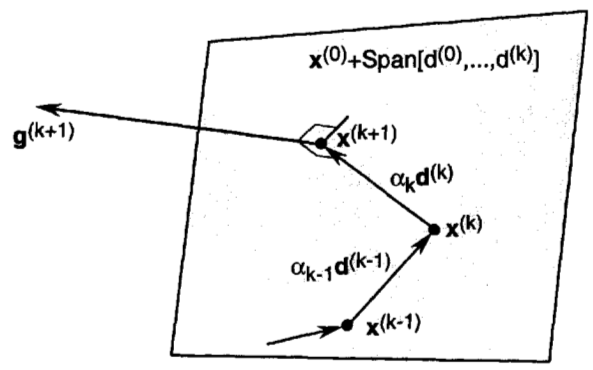
\includegraphics[scale=0.5]{orhtog}
\centering
\caption{Πόρισμα 2.2 - Καθετότητα διανυσμάτων}
\end{figure}


\subsection{Conjugate Gradient}  
O αλγόριθμος $conjugate$ $gradient$ δεν χρησιμοποιεί ήδη υπολογισμένες κατευθύνσεις αντιθέτως τις υπολογίζει καθώς "τρέχει".

Σε κάθε στάδιο του αλγορίθμου η εκάστοτε κατέυθυνση υπολογίζεται ως ένας γραμμικός συνδιασμός της προηγούμενης κατεύθυνσης και του τρέχον gradient, έτσι ώστε όλες οι κατευθύνσεις να είναι $Q-conjugate$ \ref{qcon}.

Oμοίως με πριν θα παρουσιάσουμε τα βήματα του παραπάνω αλγορίθμου :

Αρχικά θεωρούμε την τετραγωνική συνάρτηση 
\begin{align*}
f(\textbf{x})=\frac{1}{2}\textbf{x}^TQ\textbf{x}-\textbf{x}^Tb, \hspace{0.1cm} Q=Q^T>0
\end{align*}
H πρώτη κατεύθυνση αναζήτης που θα ψάξουμε να βρούμε για αρχικό σημείο $\textbf{x}^{(0)}$ θα είναι στην κατεύθυνση \textbf{steepest descent}. Επόμενως θα έχουμε :
\begin{align}
\textbf{d}^{(0)} = -\textbf{g}^{(0)} = -\nabla f(\textbf{x}^{(0)})
\end{align}
Άρα για την πρώτη επανάληψη λαμβάνουμε το διάνυσμα :
\begin{align}
\textbf{x}^{(1)} = \textbf{x}^{(0)} + a^{(0)}\textbf{d}^{(0)}\\
a^{(0)} = -\frac{\textbf{g}^{(0)T}\textbf{d}^{(0)}}{\textbf{d}^{(0)T}Q\textbf{d}^{(0)}}
\end{align}
Έπειτα συνεχίζουμε τον αλγόριθμο στην κατέυθυνση \textbf{d}$^{(1)}$ που θα είναι $Q-conjugate$ στην \textbf{d}$^{(0)}$. Επομένως επιλέγουμε την κατεύθυνση \textbf{d}$^{(1)}$ ως ένα γραμμικό συνδυασμό των \textbf{d}$^{(0)}$ και \textbf{g}$^{(1)}$. Επομένως όταν φτάσουμε στο (k+1)-βήμα θα έχουμε τον τύπο :
\begin{align}
\textbf{d}^{(k+1)} = -\textbf{g}^{(k+1)} + \beta _k\textbf{d}^{(k)}.
\end{align}
όπου οι συντελεστές $\beta _k$ δίνονται από τον ακόλουθο τύπο
\begin{align}
\beta _k = \frac{\textbf{g}^{(k+1)T}Q\textbf{d}^{(k)}}{\textbf{d}^{(k)T}Q\textbf{d}^{(k)}}
\end{align}

\begin{cor}
Οι κατευθύνσεις \textbf{d}$^{(0)}$,\textbf{d}$^{(1)}$,...,\textbf{d}$^{(n-1)}$ στον $conjugate$ $gradient$ αλγόριθμο είναι $Q-conjugate$.
\end{cor}
\begin{exmp}
Έστω ότι θέλουμε να βρούμε το ολικό ελάχιστο με χρήση του αλγορίθμου conjugate gradient , της συνάρτησης 
\begin{align*}
f(x_1,x_2,x_3) = \frac{3}{2}x_1 ^2 + 2x_2 ^2 + \frac{3}{2}x_3 ^2 + x_1x_3+2x_2x_3-3x_1-x_3,
\end{align*}
με αρχικό σημείο \textbf{x}$^{(0)} = [0,0,0]^T$.

\textbf{Λύση}\\
Αρχικά θα παραστίσουμε την f στη μορφή $f(\textbf{x})=\frac{1}{2}\textbf{x}^TQ\textbf{x}-\textbf{x}^Tb$, όπου :
\begin{align*}
Q = \begin{bmatrix}
3 & 0 & 1\\
0 & 4 & 2\\
1 & 2 & 3
\end{bmatrix}, \hspace{0.2cm} b=\begin{bmatrix}
3\\
0\\
1
\end{bmatrix}
\end{align*}
Στη συνέχεια υπολογίζουμε το gradient της συνάρτησης
\begin{align*}
\textbf{g}(\textbf{x}) = \nabla f(\textbf{x}) = \begin{bmatrix}
3x_1 + x_3 - 3\\
4x_2 + 2x_3\\
x_1+2x_2+3x_3-1
\end{bmatrix}
\end{align*}
Επομένως βρίσκοντας τα απαραίτητα μεγέθη για τον υπολογισμό της πρώτης επανάληψης, θα έχουμε :
\begin{align*}
\textbf{g}^{(0)} = [-3, 0, -1]^T,\\
\textbf{d}^{(0)} = -\textbf{g}^{(0)},\\
a^{(0)} = -\frac{\textbf{g}^{(0)T}\textbf{d}^{(0)}}{\textbf{d}^{(0)T}Q\textbf{d}^{(0)}} = \frac{5}{18},\\
\textbf{x}^{(1)} = [0.8333, 0, 0.2778]^T
\end{align*}
Στη συνέχεια του αλγορίθμου υπολογίζουμε διαδοχικά :
\begin{align*}
\textbf{g}^{(1)} = \nabla f(\textbf{x}^{(1)}) = [-0.2222, 0.5556, 0.6667]^T,\\
\beta _0 = \frac{\textbf{g}^{(1)T}Q\textbf{d}^{(0)}}{\textbf{d}^{(0)T}Q\textbf{d}^{(0)}} = 0.08025
\end{align*}
H νέα κατεύθυνση θα είναι 
\begin{align*}
\textbf{d}^{(1)} = -\textbf{g}^{(1)} + \beta _0 \textbf{d}^{(0)} = [0.4630, -0.5556, -0.5864]^T,\\
a^{(1)} = -\frac{\textbf{g}^{(1)T}\textbf{d}^{(1)}}{\textbf{d}^{(1)T}Q\textbf{d}^{(1)}} = 0.2187
\end{align*}
Έτσι βρίσκουμε στη δεύτερη επανάληψη το διάνυσμα :
\begin{align*}
\textbf{x}^{(2)} = \textbf{x}^{(1)} + a^{(1)}\textbf{d}^{(1)} = [0.9346, -0.1215, 0.1495]^T
\end{align*}
H διαδικασία του αλγορίθμου συνεχίζεται με ανάλογο τρόπο.
\end{exmp}


\section{Μέθοδοι Ολικής Βελτιστοποίησης}
\subsection{Nelder-Mead}
\begin{defn}
Στη γεωμετρία ο όρος \textbf{Simplex} αποτελεί γενίκευση της έννοιας του τριγώνου ή του τετραέδρου για αυθέραιτες διαστάσεις. Γενικότερα ένα \textbf{k-Simplex} αποτελεί ένα n-διάστατο γεωμετρικό πολύτοπο\footnote{\url{https://en.wikipedia.org/wiki/Polytope}} που είναι η κυρτή θήκη n+1 κορυφών. Πιο τυπικά έστω n+1 σημεία-κορυφές $x_0,x_1,...,x_n \in \mathbb{R}^n$ ανα δύο γραμμικώς ανεξάρτητα. Τότε το Simplex που ορίζεται από αυτά τα σημεία είναι το σύνολο :
\begin{align}
C = \{\theta _0 x_0 + \theta _1 x_1 + ...  + \theta _n x_n | \sum_{i=0}^{n}\theta _i = 1, \hspace{0.1cm} \theta _i \geq 0 \hspace{0.1cm} \forall i\}
\end{align}
\end{defn}

H μέθοδος \textbf{Nelder Mead} \cite{kelley1999iterative}  προτάθηκε από τους  John Nelder και Roger Mead το (1965). Είναι μια αριθμητική μέθοδος που χρησιμοποιείται για εύρεση του ελάχιστου ή μέγιστου μιας αντικειμενικής συνάρτησης. Εφαρμόζεται κυρίως σε μη γραμμικά προβλήματα βελτιστοποίησης για τα οποία πιθανόν δε γνωρίζουμε τις παραγώγους. 

Ο αλγόριθμος μπορεί να επεκταθεί σε προβλήματα ελαχιστοποίησης με περιορισμούς με την προσθήκη μιας συνάρτησης ποινής (\textbf{penalty function}).
Η μέθοδος χρησιμοποιεί τη διατήρηση ενός Simplex S. Το Simplex που διατηρείται κατα τη διάρκεια του αλγορίθμου μπορεί να θεωρηθεί ως ένα πολύγωνο με n+1 κορυφές . Για n=2 θα έχουμε ένα τρίγωνο όπου ο αλγόριθμος Nelder-Mead μπορεί να γίνει εύκολα αντιληπτός.

Οι κορυφές $\{x_i\}_{i=1}^n$ είναι διατεταγμένες σύμφωνα με τις συναρτησιακές τιμές
\begin{align*}
f(x_1) \leq f(x_2) \leq ... \leq f(x_{n+1}) 
\end{align*}
όπου $x_1$ αποτελεί την καλύτερη κορυφή (\textbf{best vertex}) και η $x_{n+1}$ τη χειρότερη (\textbf{worst vertex}).

Eάν υπάρχουν κορυφές με την ίδια τιμή με τη $x_1$ τότε η καλύτερη κορυφή δεν είναι μοναδική. Το σκεπτικό του αλγορίθμου είναι η αντικατάσταση της χειρότερης κορυφής $x_{n+1}$ με ένα νέο σημείο της μορφής 
\begin{align*}
x(\mu) = (1+\mu)\overline{x} - \mu x_n
\end{align*}
όπου $\overline{x}$ είναι το κεντροειδές της κυρτής θήκης των σημείων $x_0$ έως $x_{n-1}$ και ορίζεται ως 
\begin{align*}
\overline{x} = \frac{1}{n}\sum_{i=i}^{n}x_i
\end{align*}


Συγκεκριμένα ο αλγόριθμος Νelder-Mead για ένα Simplex  με 3 κορυφές $u,v,w$ και αντίστοιχες συναρτησιακές τιμές $f(u),f(v),f(w)$ ακολουθεί τα παρακάτω βήματα.

\begin{figure}[h]
\centering
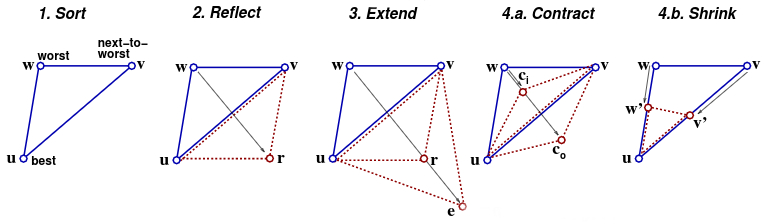
\includegraphics[scale=0.64]{nelder1b}
\caption{Τα βήματα του αλγορίμου Nelder-Mead (για n = 2) \cite{gavin2013nelder}.}
\end{figure}

\begin{enumerate}
\item \label{it1} Διάταξη (\textbf{Sort}) των κορυφών $u,v,w$ τ.ω. $f(u)<f(v)<f(w)$. 

To σημείο u αποτελεί  την "καλύτερη" κορυφή και το w τη "χειρότερη" κορυφή.
\item \label{it2} "Αντανάκλαση" (\textbf{Reflect}) της χειρότερης κορυφής w  από το κεντροειδές $\overline{x}$ των σημείων που μένουν u,v και υπολογισμός του σημείου αντανάκλασης r όπως και της συναρτησιακής τιμής αυτού.

Εάν $f(u)<f(r)<f(v)$ τότε αντικαθιστώ το $w$ με το $r$ και πηγαίνω στο βήμα \ref{it5}.
\item \label{it3} Εάν $f(r)<f(u)$, άρα έχω νέα καλύτερη κορυφή, τότε "επεκτείνω" (\textbf{Εxtend}) το $r$, πέρα από το μέσο όρο των $u,v$ σε ένα σημείο $e$ και υπολογίζω το $f(e)$.
\begin{itemize}
\item  Eάν ισχύει ότι $f(e) < f(r)$, τότε αντικαθιστώ τη χειρότερη κορυφή $w$ με το σημείο $e$ και πηγαίνω στο βήμα \ref{it5}
\item Διαφορετικά αντικαθιστώ το $w$ με το σημείο αντανάκλασης $r$ και πηγαίνω στο βήμα \ref{it5}.
\end{itemize}
\item \label{it4} Εάν οι ανισότητες των βημάτων \ref{it2} και \ref{it3} δεν ικανοποιούνται, τότε σίγουρα το $r$ είναι χειρότερη κορυφή από το $v$ δηλαδή $f(v)<f(r)$, και πιθανόν να υπάρχει μικρότερη συναρτησιακή τιμή μεταξύ των σημείων $w$ και $r$. 

Έτσι κάνω σύμβαση (\textbf{Contract}) για το $w$ με ένα σημείο $c$ το οποίο βρίσκεται μεταξύ των $w$ και $r$, υπολογίζοντας και το $f(w)$. Γενικά κάποιες καλές τιμές για το c είναι 1/4 και 3/4 της απόστασης από το $w$ στο $r$. Τα σημεία αυτά καλούνται \textbf{εσωτερικό} και \textbf{εξωτερικό} σημείο σύμβασης, και συμβολίζονται αντίστοιχα $c_i$ και $c_o$.
\begin{itemize}
\item Eάν $min\{f(c_i),f(c_0)\} < f(v)$ τότε αντικαθιστώ το $w$ με το καλύτερο από τα σημεία σύμβασης $c_i$ και $c_0$.
\item Διαφορετικά γίνεται "συστολή" του Simplex στην καλύτερη κορυφή $u$ και πηγαίνω στο βήμα \ref{it5}.
\end{itemize}
\item \label{it5} Έλεγχος σύγκλισης.

Το Simplex συγκλίνει εάν είναι όπως λέμε "επαρκώς" μικρό και αν συναρτησιακές τιμές βρίσκονται "επαρκώς" κοντά. H επάρκεια καθορίζεται από τις ακρίβειες $\varepsilon _x$ και $\varepsilon _f$ αντίστοιχα. Ακολουθούν οι απαραίτητες συνθήκες για τη σύγκλιση.
\begin{align*}
2 \underset{n=2}{max}|\frac{[u,v] - [v,w]}{[u,v] + [v,w]}| < \varepsilon _x , \hspace{0.25cm} 2\underset{n\geq 2}{max}|\frac{\textbf{S}(:, 1 : n) − \textbf{S}(:, 2 : n + 1)}{\textbf{S}(:, 1 : n) + \textbf{S}(:, 2 : n + 1)}| < \varepsilon _x
\end{align*}
και οι αντίστοιχες συνθήκες για τις συναρτησιακές τιμές :
\begin{align*}
|\frac{f (w) − f (u)}{f (u) + 10^{-9}}| _{n=2} < \varepsilon _f , \hspace{0.25cm} |\frac{f (n + 1) − f (1)}{f (1) + 10^{−9}}|_{n\geq 2} < \varepsilon _f
\end{align*}
Όπου \textbf{S}$(:,1:n)$ αντιστοιχεί στο Simplex που σχηματίζεται κατά την εκτέλεση του αλγορίθμου, από το πρώτο μέχρι το n-σημείο.

\begin{itemize}
\item Άν οι παραπάνω συνθήκες ισχύουν τότε έχουμε σύγκλιση και ο αλγόριθμος τερματίζει.
\item Άν το πλήθος των επαναλήψεων έχει ξεπεράσει κάποιο όριο τότε ο αλγόριθμος τερματίζει.
\end{itemize}
\end{enumerate}

\begin{figure}[h]
\centering
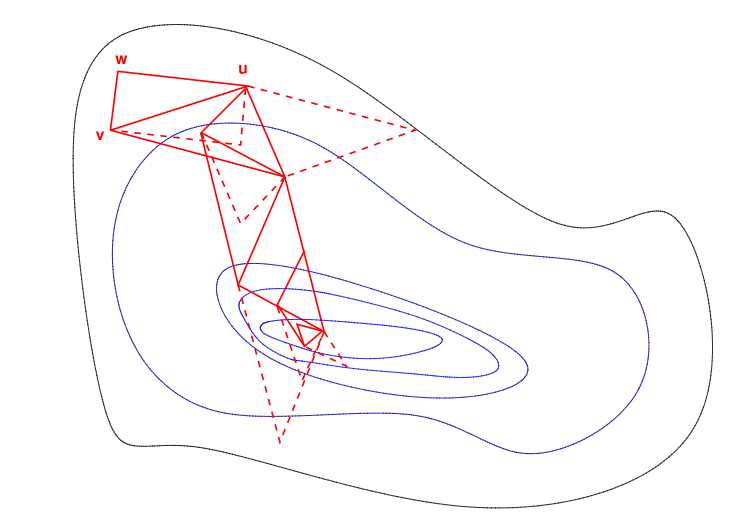
\includegraphics[scale=0.6]{nelder2}
\caption{Η ακολουθία επτά βημάτων του αλγορίθμου Nelder-Mead. Οι διακεκομμένες γραμμές δείχνουν τις προσπάθειες βημάτων ανάκλασης \cite{gavin2013nelder}.}
\end{figure}


%\subsection{Στοχαστική Ανόπτηση}
\subsection{Basin Hopping}
% http://stackoverflow.com/questions/22207372/example-to-understand-scipy-basin-hopping-optimization-function
Ο αλγόριθμος αυτός έρχεται από τον χώρο της φυσικοχημείας, όπου οι επιστήμονες μελετάνε την ευστάθεια μοριακών συστημάτων ως το ελάχιστο της ολικής τους ενέργειας. Όσο αυξάνεται η πολυπλοκότητα των  μοριακών δομών όμως, τόσο πιο δύσκολο είναι να βρει κανείς ολικά ελάχιστα του ενεργιακού επίπεδου του κάθε συστύματος, μιας και στις χαμηλές ενέργειες (θερμοκρασίες) είναι πολύ πιθανό το σύστημα να ισορροπήσει σε κάποιο τοπικό ελάχιστο. Η ενεργειακή συνάρτηση είναι γνωστή στον χώρο της φυσικοχημείας και ως δυναμικό Lennard-Jones \footnote{\url{https://en.wikipedia.org/wiki/Lennard-Jones_potential}} και στην περίπτωσή  μας που έχουμε πολυμοριακά συστήματα δίνεται από την ακόλουθη σχέση (Lennard-Jones cluster \cite{Iwamatsu_2004}):

\begin{equation}
	E_n = 2\sum^n_{i=1}\sum^n_{j=1} ( \frac{1}{r^{12}_{ij}} - \frac{1}{r^6_{ij}} )
\end{equation}

, όπου n είναι ο αριθμός των σωματιδίων του συστήματός (cluster) υπό μελέτη, $E_n$ η ενέργεια του $n^{\textnormal{στού}}$ σωματιδίου, και $r_{ij}$ η ευκλείδια απόσταση μεταξύ των σωματιδίων i και j.

Για αυτό τον λόγο οι Wales κ.α. \cite{Wales_1997} ανέπτυξαν την  μέθοδο basin hopping που χρησιμοποιεί κάποια από τις μεθόδους εύρεσης τοπικών ελαχίστων που ήδη έχουμε αναφέρει για να βρούμε όλα τα τοπικά ελάχιστα της ενεργειακής συνάρτησης, και έπειτα με το κριτήριο Metropolis, η λύση μας μεταβαίνει στο επόμενο ενεργειακό επίπεδο ή παραμένει εκεί που είναι.

Στο σχήμα που ακολουθεί βλέπουμε με την μπλε ομαλή καμπύλη την ενεργειακή συνάρτηση Е όπως φαίνεται, ενώ η μετασχηματισμένη ενέργεια $\tilde{E}$ φαίνεται με τα πράσινα κατώφλια (basins), που ορίζουν τα τοπικά ελάχιστα της αρχικής συνάρτησης Е.

\begin{figure}[h]
	\centering
	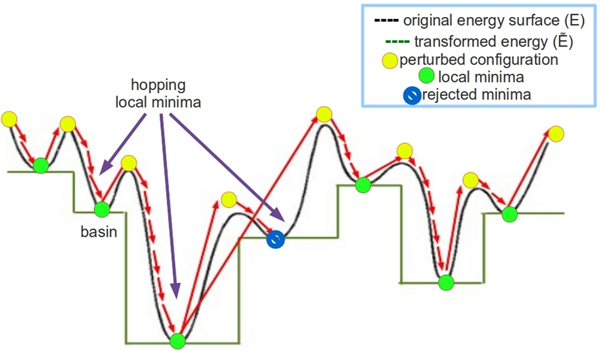
\includegraphics[scale=0.7]{basin-hoping2}
    \caption{Εικόνα της λειτουργίας του αλγορίθμου basin hopping \cite{Hashmi_2013}}
\end{figure}

Το κριτήριο μετάβασης από το ένα τοπικό ελάχιστο σε κάποιο άλλο, το δίνει το κριτήριο του Metropolis \cite{Wille_1987} που μετακινεί τυχαία την λύση/σωματίδιο i κατά $\Delta \textbf{r}_i$ αν η μεταβολή της ολικής ενέργειας  $\Delta E = E(\textbf{r}_1,...,\textbf{r}_i + \Delta\textbf{r}_i,...,r_N) - E(\textbf{r}_1,...,\textbf{r}_i,...,\textbf{r}_N)$ είναι αρνητική ή μηδέν. Δηλαδή αν πάει σε μικρότερο τοπικό ελάχιστο ή μείνει στο ίδιο. Αν η μεταβολή της ενέργειας είναι θετική, τότε το σωματίδιο έχει πιθανότητα $exp(-\Delta E/T)$ να αλλάξει θέση, με Т να υποδηλώνει την θερμοκρασία.  

Το λογικό διάγραμμα του αλγόριθμου basin hopping είναι το ακόλουθο, όπου ως κριτήριο τερματισμού δίνουμε τον μέγιστο αριθμό των μεταβάσεων που θέλουμε να κάνει η λύση της συναρτησης υπό βελτιστοποίηση.

\begin{figure}[h]
	\centering
	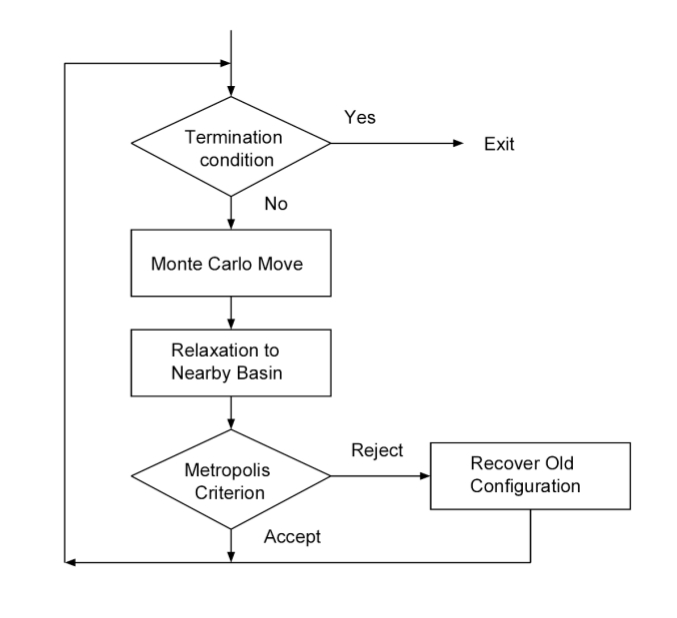
\includegraphics[scale=0.7]{hbasinflow}
    \caption{Το λογικό διάγραμμα του αλγορίθμου Basin Hopping (Iwamatsu et al \cite{Iwamatsu_2004})}
\end{figure}

%%%%%%% ΚΕΦΑΛΑΙΟ 3
\newpage
\chapter{Εισαγωγή στα Jupyter Notebooks}
\section{Οδηγίες εγκατάστασης}
\subsection{Στο λειτουργικό σύστημα MS Windows}

Σε αυτό το λειτουργικό σύστημα αρκεί ο χρήστης να εγκαταστήσει το πακέτο της Python Anaconda, το οποίο εγκαθιστά όλα τα απαραίτητα πακέτα, την IPython, καθώς και τις βιβλιοθήκες NumPy, SciPy, Pandas, Matplotlib. Ό,τι δηλαδή χρειάζεται κανείς για να αναπαραγάγει τα αποτελέσματα αυτής της εργασίας.

Για να εγκαταστήσει κανείς το Anaconda θα χρειαστεί να πάει στον 
\href{https://www.continuum.io/downloads#linux}{ιστότοπο}
της Anaconda και να επιλέξει την έκδοση 2.7 της Python ("Python 2.7 version").

Ἐπειτα, αφότου κατεβάσει το πακέτο για υπολογιστή 64bit, το εγκαθιστά και από την Έναρξη/Start του Windows πηγαίνει στα προγράμματα, στον φάκελο Anaconda.

\subsection{Στο λειτουργικό σύστημα GNU/Linux}

Οι τρεις πιο διαδεδομένες «γεύσεις» (flavors) αυτού του λειτουργικού συστήματος είναι σύμφωνα  με τον ιστότοπο Distrowatch \footnote{\url{https://distrowatch.com/dwres.php?resource=major}} το Mint, το Ubuntu και το Debian. 

Το Mint είναι παράγωγο GNU/Linux του Ubuntu. Ενώ το Ubuntu είναι παράγωγο του Debian. Συνεπώς και τα τρία χρησιμοποιούν το ίδιο πρόγραμμα εγκατάστασης πακέτων, to apt-get. Ο κώδικας αυτής της εργασίας έχει δοκιμαστεί και τρέχει τόσο σε Ubuntu ὀσο και σε Lubuntu, οπότε αναμένουμε πως θα τρέχει και σε Debian και Mint.

Η εγκατάσταση των Jupyter Notebooks λοιπόν αφορά και τα τρία (Mint, Ubuntu, Debian), αλλά προτείνουμε να διαλέξετε κάποιο από τα Ubuntu (Ubuntu, Lubuntu, Kubuntu). Οι διαδικασίες που ακολουθούν έχουν ως αυστηρό προαπαιτούμενο ο υπολογιστής μας να είναι συνδεδεμένος στο διαδίκτυο.

\subsubsection{Εγκατάσταση της Python}

Ανοίγουμε ένα τερματικό εντολών. Έπειτα γράφουμε:
\begin{lstlisting}[extendedchars=true,language=bash]
	sudo apt-get install python2.7 -y
\end{lstlisting}

Θα μας ζητήσει τον κωδικό του username, και αφότου τον δώσουμε θα εγκαταστήσει την python2.7 και όλα τα σχετικά.

\subsubsection{Εγκατάσταση του pip}

Εφόσον εγκαταστήθηκε η Python, ήδη υπάρχει και το pip, αλλά σε παλαιότερη έκδοση. Για να κατεβάσουμε την τελευταία έκδοση γράφουμε στο τερματικό:
\begin{lstlisting}[extendedchars=true,language=bash]
pip install -U pip setuptools
\end{lstlisting}

\subsubsection{Εγκατάσταση του virtual environment}
Μια καλή τακτική όταν κανείς δουλεύει με τις βιβλιοθήκες της Python σε κάποιο project είναι να φτιάξει ένα virtual environment για το συγκεκριμένο project το οποίο δεν θα επικοινωνεί με τα υπόλοιπα πακέτα της Python που είναι ήδη εγκατεστημένα στον υπολογιστή.

Για να εγκαταστήσουμε το virtual environment, και να δημιουργήσουμε ένα φάκελο με τις βιβλιοθήκες μας για ένα project με όνομα NumericalOptimization και για να το ενεργοποιήσουμε, γράφουμε στο τερματικό μας:
\begin{lstlisting}[extendedchars=true,language=bash]
pip install virtualenv
virtualenv NumericalOptimization
source NumericalOptimization/bin/activate
\end{lstlisting}

Τώρα η γραμμή εντολών μας θα πρέπει να φαίνεται κάπως έτσι:
\begin{center}
	\texttt{(NumericalOptimization)milia@Newton\$\_}
\end{center}
για έναν χρήστη με όνομα \textit{milia} και με όνομα υπολογιστή \textit{Newton}. Η παρένθεση \textit{(Numerical} \textit{Optimization)} μπροστά από το όνομα του χρήστη δείχνει πως χρησιμοποιούμε το περιβάλλον της Python ονόματι «NumericalOptimization».

\subsubsection{Εγκατάσταση των Jupyter Notebooks, NumPy, SciPy, Matplotlib}

Για να εγκαταστήσουμε τα παραπάνω θα πρέπει να ακολουθήσουμε τις ακόλουθες ενέργειες πρώτα:
\begin{lstlisting}[extendedchars=true,language=bash]
sudo apt-get install build-essential python-dev
sudo apt-get install libblas-dev liblapack-dev libatlas-base-dev gfortran
\end{lstlisting}

Τώρα μπορούμε να εγκαταστήσουμε τα προγράμματά μας με το pip:
\begin{lstlisting}[extendedchars=true,language=bash]
pip install scipy numpy matplotlib jupyter
\end{lstlisting}

\subsubsection{Αναβάθμιση των προγραμμάτων που εγκαταστήσαμε με το pip}

Δεν είναι σπάνιο φαινόμενο να θελήσουμε να ξαναπιάσουμε το συγκεκριμένο project μετά από μερικούς μήνες. Μέχρι τότε θα έχουν βγει νέες εκδόσεις των πακέτων που θα'χουμε ήδη κατεβάσει. Για να κατεβάσουμε τις νέες εκδόσεις όλες μαζί υπάρχει ένα εξαίρετο εργαλείο, το \texttt{pip-review} το οποίο και καλό είναι να εγκαταστήσουμε:
\begin{lstlisting}[extendedchars=true,language=bash]
pip install pip-review
\end{lstlisting}

Έτσι, για την ανανέωση των προγραμμάτων της Python με τις τελευταίες εκδόσεις τους αρκεί να γράψουμε στο τερματικό:
\begin{lstlisting}[extendedchars=true,language=BASH]
pip-review --local --interactive
\end{lstlisting}

και να επιλέξουμε την επιλογή "All" \footnote{\url{http://stackoverflow.com/questions/2720014/upgrading-all-packages-with-pip}}.

\section{Οδηγίες χρήσης}

Ωραία, τώρα που εγκαταστήσαμε τα Jupyter Notebooks πώς τα ξεκινάμε; Το σημαντικό τους προσόν είναι ότι τρέχουν στον browser μας. 

\subsection{Στо MS Windows}

Για να ανοίξουμε ένα Jupyter Notebook στο λειτουργικό σύστημα Windows 7 ακολουθούμε τις ακόλουθες ενέργειες:

\begin{enumerate}
\item Πηγαίνουμε στο κουμπί Start/Έναρξη
\item Πηγαίνουμε στο All Programms/Προγράμματα
\item Βρίσκουμε τον φάκελο Anaconda και τον πατάμε με αριστερό κλικ του ποντικιού
\item Επιλέγουμε την εφαρμογή Jupyter Notebook και την πατάμε με το αριστερό κλικ
\item Παρατηρούμε πως άνοιξε ένα νέο υποπαράθυρο (tab) στον browser μας μαζί και με ένα μικρό παράθυρο εντολών (command line). 
\item Αγνοούμε το παράθυρο εντολών και πηγαίνουμε στο tab του browser που άνοιξε
\item Πατάμε New και επιλέγουμε Python 2, κάτω από τον τίτλο Notebooks.
\end{enumerate}

Αν όλα έχουν πάει καλά, και τα Jupyter Notebooks εχουν ρυθμιστεί έτσι ώστε να ανοίγουν σε έναν φάκελο που έχετε δικαιώματα γραφής (write permissions) στον σκληρό, θα βλέπετε ένα κενό Jupyter Notebook στο συγκεκριμένο tab, με ένα κενό κελί όπου μπορείτε να γράψετε κάποιον κώδικα Python.

Αφότου γράψετε κάποια εντολή σε γλώσσα Python στο συγκεκριμένο κελί, για την εκτέλεσή της πατήστε Shift + Enter, οπως στην Mathematica. Τα Jupyter Notebooks ξεκίνησαν ως προέκταση των IPython Notebooks που εφευρέθηκαν από έναν ερευνητή που ήθελε να μεταφέρει την ευκολία των Mathematica Notebooks στην Python. Περισσότερες πληροφορίες για την ιστορία των Jupyter Notebooks και της IPython μπορείτε να βρείτε στην wikipedia\footnote{\url{https://en.wikipedia.org/wiki/IPython}}.

\subsection{Στο Ubuntu}

Ανοίγουμε ένα τερματικό εντολών. Μπαίνουμε στο virtual environment που έχουμε φτιάξει όπου είναι εγκατεστημένο και το Jupyter Notebook:

\begin{lstlisting}[extendedchars=true,language=bash]
source NumericalOptimization/bin/activate
\end{lstlisting}

Τώρα πάμε στο directory που θέλουμε να δουλέψουμε ή όπου υπάρχει το notebook που φτιάξαμε την  προηγούμενη φορά. Έστω πως βρίσκεται στο home directory \texttt{/home/milia/}. Οπότε μπορούμε να γράψουμε:
\begin{lstlisting}[extendedchars=true,language=bash]
cd
jupyter notebook
\end{lstlisting}

και θα δούμε στο τερματικό
\begin{lstlisting}[extendedchars=true,language=bash]
[I 21:45:24.587 NotebookApp] Writing notebook server cookie secret to
/run/user/1000/jupyter/notebook_cookie_secret
[I 21:45:28.190 NotebookApp] Serving notebooks from local directory:
/home/milia/
[I 21:45:28.191 NotebookApp] 0 active kernels 
[I 21:45:28.191 NotebookApp] The Jupyter Notebook is running at:
http://localhost:8888/
[I 21:45:28.191 NotebookApp] Use Control-C to stop this server and
shut down all kernels (twice to skip confirmation).
\end{lstlisting}

Λογικά θα ανοίξει αυτόματα τον ορισμένο ως κύριο browser μας στην διεύθυνση \texttt{http://localhost:8888/}, αλλιώς μπορείτε να το αντιγράψετε και επικολλήσετε μόνοι σας στον browser που έχετε ανοιχτό.

\section{Η βιβλιοθήκη SciPy}

Η βιβλιοθήκη \href{https://www.scipy.org/about.html}{SciPy}\footnote{\url{https://www.scipy.org/about.html}} ανήκει στην συλλογή πακέτων για επιστημονικούς υπολογισμούς στην γλώσσα Python, γνωστή και ως SciPy Stack. Εμείς θα ασχοληθούμε μόνο με την βιβλιοθήκη SciPy και θα αναφερθούμε και στην βιβλιοθήκη NumPy.

Από την SciPy μας ενδιαφέρει η συλλογή αλγορίθμων που αφορούν επίλυση προβλημάτων βελτιστοποίησης. Η κλάση αυτών των μεθόδων ονομάζεται optimize \footnote{\url{https://docs.scipy.org/doc/scipy-0.18.1/reference/tutorial/optimize.html}}. Όπως μπορεί να δει κανείς στο εγχειρίδιο χρήσης (tutorial) στον σχετικό σύνδεσμο, αυτή η κλάση περιέχει όλες τις μεθόδους τις οποίες εξετάζουμε σε αυτή την εργασία. Μια αναλυτική λίστα για τις συγκεκριμένες μεθόδους υπάρχει σε \href{https://docs.scipy.org/doc/scipy-0.18.1/reference/optimize.html#module-scipy.optimize}{αυτόν}  τον σύνδεσμο.

Πιο συγκεκριμένα, από την κλάση $\texttt{scipy.optimize}$ θα χρησιμοποιήσουμε τις μεθόδους $\texttt{minimize}$ και $\texttt{basinhopping}$. Η πρώτη μέθοδος βρίσκει το ελάχιστο δεδομένης συνάρτησης ανάλογα με την μέθοδο που θα επιλέξουμε (Nelder-Mead, Powell, CG, Newton-CG, BFGS) ενώ η δεύτερη χρησιμοποιεί τον στοχαστικό αλγόριθμο Basin Hopping για την εύρεση του ελάχιστου μιας δεδομένης συνάρτησης.

Περισσότερες λεπτομέρειες για το πώς λειτουργεί η  $\texttt{minimize}$ και η  $\texttt{basinhopping}$ μπορούν να βρεθούν στον κώδικά τους που υπάρχει διαθέσιμος στο διαδίκτυο\footnote{\url{https://docs.scipy.org/doc/scipy-0.18.1/reference/generated/scipy.optimize.minimize.html\#scipy.optimize.minimize}}
\footnote{\url{https://docs.scipy.org/doc/scipy-0.18.1/reference/generated/scipy.optimize.basinhopping.html\#scipy.optimize.basinhopping}}. Στην παρούσα εργασία θα εξετάσουμε τις συγκεκριμένες μεθόδους όσον αφορά την απόδοσή τους σε συγκεκριμένα προβλήματα ως κλειστά κουτιά (black boxes).

H NumPy στην οποία αναφερθήκαμε πιο πάνω και την οποία καλούμε στον κώδικά μας ($\texttt{import numpy as np}$) περιέχει όλες τις βασικές συναρτήσεις που θα χρειαστούμε για την υλοποίηση των προβλημάτων προς επίλυση.
%%%%%%%%%%%%%%%%%%%%%%%%%%%%%%%%%%%%%%%%%%%%%%%%%%%%%%%%%
\newpage
\chapter{Πειραματική διαδικασία}

\section{Παρουσίαση των προβλημάτων προς επίλυση}
Από την εργασία των More et al \cite{More1981} πήραμε τα ακόλουθα προβλήματα ώστε να ελέγξουμε την απόδοση των υλοποιήσεων των παραπάνω αλγορίθμων της βιβλιοθήκης SciPy.
%\subsection{Με μαθηματικούς φορμαλισμούς}
\begin{enumerate}
\item \textbf{Συνάρτηση Badly scaled του Powell}
\begin{align}
f(\textbf{x}) = (10^4x_1x_2-1)^2 + (e^{-x_1}+e^{-x_2} - 1.0001)^2
\end{align}
όπου  \textbf{x}$_0 = (0,1)^T$,\hspace{0.1cm} \textbf{x}$^*=(1.098\times10^{-5}, 9.106)^T$, \hspace{0.1cm} $f($\textbf{x}$^*)=0$.

\begin{lstlisting}[extendedchars=true,caption="Η συνάρτηση Powell σε κώδικα Python",language=python]
f1a = lambda x: (10**4)*x[0]*x[1] - 1
f2a = lambda x: (m.exp(-x[0]) + m.exp(-x[1]) - 1.0001)
powell_func = lambda x: square(f1a(x)) + square(f2a(x))
powell_f = lambda x: powell_func([x[0],x[1]])

def powell_f2(x):
    f = (square((10**4)*x[0]*x[1] - 1) + square((m.exp(-x[0]) + 
    	m.exp(-x[1]) - 1.0001)))
    df = np.zeros(2)
    df[0] = 2*((10**4)*x[0]*x[1] - 1)*(10**4)*x[1] -2*m.exp(-x[0])
    df[1] = 2*((10**4)*x[0]*x[1] - 1)*(10**4)*x[0] -2*m.exp(-x[1])
    return f,df
\end{lstlisting}

\item \textbf{Συνάρτηση Badly scaled του Brown }
\begin{align}
f(\textbf{x}) = (x_1-10^6)^2+(x_2-2\times 10^{-6}+(x_1x_2-2))^2
\end{align}
όπου  \textbf{x}$_0 = (1,1^T)$,\hspace{0.1cm} \textbf{x}$^*=(10^6, 2\times 10^6)^T$, \hspace{0.1cm} $f($\textbf{x}$^*)=0$.

\begin{lstlisting}[extendedchars=true,caption="Η συνάρτηση Brown σε κώδικα Python",language=python]
f1b = lambda x: x[0] - 10**6
f2b = lambda x: x[1] - 2*10**(-6)
f3b = lambda x: x[0]*x[1] - 2

brown_func = lambda x: (square(f1b(x)) + square(f2b(x)) + 
					   square(f3b(x)))

def brown_func2(x):
    f = brown_func(x)
    df = np.zeros(2)
    df[0] = 2*(x[0] - 10**6) + 0 + 2*(x[0]*x[1] - 2)*x[1] 
    df[1] = 0 + 2*(x[1] - 2*10**(-6)) + 2*(x[0]*x[1] - 2)*x[0]
    return f,df

\end{lstlisting}

\item \textbf{Συνάρτηση του Beale}
\begin{align}
f(\textbf{x}) = (1.5-x_1(1-x_2))^2+(2.25-x_1(1-x_2^2))^2+(2.625-x_1(1-x_2^3))^2
\end{align}
όπου  \textbf{x}$_0 = (1,1)^T$,\hspace{0.1cm} \textbf{x}$^*=(3, 0.5)^T$, \hspace{0.1cm} $f($\textbf{x}$^*)=0$.
\begin{lstlisting}[extendedchars=true,caption="Η συνάρτηση Beale σε κώδικα Python",language=python]
const = [1.5, 2.25, 2.625]
f1c = lambda x: const[0] -x[0]*(1 - x[1]) 
f2c = lambda x: const[1] -x[0]*(1 - x[1]*x[1])
f3c = lambda x: const[2] -x[0]*(1 - x[1]*x[1]*x[1])

beal_func = lambda x: (square(f1c(x)) + square(f2c(x)) +
					  square(f3c(x)))
def beal_func2(x):
    f = beal_func(x)
    df = np.zeros(2)
    df[0] = (2*(const[0] -x[0]*(1 - x[1]))*(-(1 - x[1]))
            +2*(const[1] -x[0]*(1 - x[1]*x[1]))*(-(1 - x[1]*x[1]))
            +(2*(const[2] -x[0]*(1 - x[1]*x[1]*x[1]))*
             (-(1 - x[1]*x[1]*x[1]))))
    
    df[1] = (2*(const[0] -x[0]*(1 - x[1]))*x[0]
            +2*(const[1] -x[0]*(1 - x[1]*x[1]))*(2*x[1])
            +(2*(const[2] -x[0]*(1 - x[1]*x[1]*x[1]))*
             (3*x[1]*x[1])))
    return f,df
\end{lstlisting}

\item \textbf{Συνάρτηση ελικοειδούς κοιλάδας (Helical valey) }
\begin{align}
f(\textbf{x}) = 100(x_3-10\theta(x_1,x_2))^2+(\sqrt{x_1^2+x_2^2}-1)^2 + x_3^2\\
\theta(x_1,x_2) =
\begin{cases}
(1/2\pi) \cdot arctan(x_2/x_1) \textnormal{,  αν   } x_1 > 0\\
0.5 + (1/2\pi) \cdot arctan(x_2/x_1) \textnormal{,  αν   } x_1 < 0
\end{cases}
\end{align}
\begin{lstlisting}[extendedchars=true,caption="Η συνάρτηση Helical valey σε κώδικα Python",language=python]
def theta(x0,x1):
    if x0 > 0:
        return np.arctan(x1/x0)/PI
    if x0 < 0:
        return 0.5 + np.arctan(x1/x0)/PI
    
f1d = lambda x: 10*(x[2] - 10*theta(x[0],x[1]))
f2d = lambda x: 10*((x[0]**2 + x[1]**2)**(1/2) - 1.0)
f3d = lambda x: x[2]

def helic_func(x): return (square(f1d(x)) + square(f2d(x)) + 
						  square(f3d(x)))

def helic_func2(x):
    f = helic_func(x)
    df = np.zeros(3)
    df[0] = ( 200*(x[2] - 10*theta(x[0],x[1]))*(x[1]/(x[0]**2 + 
    		  x[1]**2)) + 20*((x[0]**2 + x[1]**2)**(1/2) 
              - 1.0)*(0.5*((x[0]**2 + x[1]**2)**(-1/2))*2*x[0])
              + 0 )
    df[1] = ( 200*(x[2] - 10*theta(x[0],x[1]))*(-x[1]/(x[0]**2 + 
    		  x[1]**2)) + 20*((x[0]**2 + x[1]**2)**(1/2) 
              - 1.0)*(0.5*((x[0]**2 + x[1]**2)**(-1/2))*2*x[1])        
              + 0 )
    df[2] = ( 20*(10*(x[2] - 10*theta(x[0],x[1]))) + 0  + 1 )
    return f,df
\end{lstlisting}

όπου  \textbf{x}$_0 = (-1,0,0)^T$,\hspace{0.1cm} \textbf{x}$^*=(1, 0,0)^T$, \hspace{0.1cm} $f($\textbf{x}$^*)=0$.

\item \textbf{Συνάρτηση του Wood}
\begin{align}
\begin{split}
f(\textbf{x}) &= 100(x_2-x_1^2)^2+(1-x_1)^2+90(x_4-x_3^2)^2+(1-x_3)^2 \\
&+10(x_2+x_4-2)^2 + 0.1(x_2-x_4)^2
\end{split}
\end{align}
όπου  \textbf{x}$_0 = (-3,-1,-3,-1)^T$,\hspace{0.1cm} \textbf{x}$^*=(1,1,1,1)^T$, \hspace{0.1cm} $f($\textbf{x}$^*)=0$.
\begin{lstlisting}[extendedchars=true,caption="Η συνάρτηση Wood σε κώδικα Python",language=python]
f1e = lambda x: (10*(x[1] - x[0]*x[0]))
f2e = lambda x: (1 - x[0])
f3e = lambda x: np.sqrt(90)*(x[3] - x[2]*x[2])
f4e = lambda x: (1 - x[2])
f5e = lambda x: np.sqrt(10)*(x[1] + x[3] - 2)
f6e = lambda x: (1/np.sqrt(10))*(x[1] - x[3])

wood_func = lambda x: (square(f1e(x)) + square(f2e(x)) + 
					  square(f3e(x)) + square(f4e(x)) + 
                      square(f5e(x)) + square(f6e(x)))
def wood_func2(x):
    f = wood_func(x)
    df=np.zeros(4)
    df[0] = 2*100*(x[1]-x[0]*x[0])*(-2*x[0]) - 2*(1-x[0])
    df[1] = 2*100*(x[1]-x[0]*x[0]) + 2*10*(x[1]+x[3]-2) 
    		+ 0.1*2*(x[1]-x[3])
    df[2] = 2*90*(x[3]-x[2]*x[2])*(-2*x[2]) - 2*(1-x[2])
    df[3] = 2*90*(x[3]-x[2]*x[2]) + 2*10*(x[1]+x[3]-2) 
    		- 2*0.1*(x[1]-x[3])
    return f,df
\end{lstlisting}

\item \textbf{Συνάρτηση του Rosenbrock}
\begin{align}
f(\textbf{x}) = 100(x_2-x_1^2)^2+(1-x_1)^2
\end{align}
όπου  \textbf{x}$_0 = (-1.2,1)^T$,\hspace{0.1cm} \textbf{x}$^*=(1, 1)^T$, \hspace{0.1cm} $f($\textbf{x}$^*)=0$.
\begin{lstlisting}[extendedchars=true,caption="Η συνάρτηση Rosenbrock σε κώδικα Python",language=python]
rosen = lambda x: scipy.optimize.rosen(x)
drosen = lambda x: scipy.optimize.rosen_der(x)

def rosen2(x):
    f = rosen(x)
    df = drosen(x)
    return f,df
\end{lstlisting}
\item \textbf{Συνάρτηση των Freudestein και Roth}
\begin{align}
\begin{split}
f(\textbf{x}) &= \{-13+x_1+[(5-x_2)x_2-2]x_2\}^2\\
&+\{-29+x_1+[(1+x_2)x_2-14]x_2\}^2
\end{split}
\end{align}
όπου  \textbf{x}$_0 = (0.5,-2)^T$,\hspace{0.1cm} \textbf{x}$^*=(5, 4)^T$, \hspace{0.1cm} $f($\textbf{x}$^*)=0$, \\
\hspace{0.1cm} $\textbf{x'}$=(11.41..., -0.8968...), \hspace{0.1cm}$f(\textbf{x'})$= 48.9842...
\begin{lstlisting}[extendedchars=true,caption="Η συνάρτηση των Freudestein και Roth σε κώδικα Python",language=python]
f1e = lambda x: -13 + x[0] + ((5-x[1])*x[1]-2)*x[1]
f2e = lambda x: -29 + x[0] + ((x[1]+1)*x[1]-14)*x[1]

fr_func = lambda x: (square(f1e(x)) + square(f2e(x)))

def fr_func2(x):
    f = fr_func(x)
    df=np.zeros(2)
    df[0] = 2*(-13 + x[0] + ((5-x[1])*x[1]-2)*x[1] 
    	   -29 + x[0] + ((x[1]+1)*x[1]-14)*x[1])
    df[1] = 2*(-13 + x[0] + ((5-x[1])*x[1]-2)*x[1])*
    	   (((5-x[1])*x[1]-2) + x[1]*(5-2*x[1])) + 
           2*(-29 + x[0] + ((x[1]+1)*x[1]-14)*x[1])*
           (((x[1]+1)*x[1]-14)+x[1]*(1 + 2*x[1]))
    return f,df

\end{lstlisting}
\end{enumerate}
%    \subsection{Με κώδικα python}
    
\section{Υλοποιήσεις υπολογισμών}
\subsection{Κλήση των βιβλιοθηκών}
    
\begin{lstlisting}[extendedchars=true,caption= Η βασική εργαλειοθήκη,language=python]
import math as m
from scipy.optimize import minimize, basinhopping
import scipy
import numpy as np
PI = np.pi

# Class for Basin-Hopping method.
class MyTakeStep(object):
    def __init__(self, stepsize=0.5):
        self.stepsize = stepsize
    def __call__(self, x):
        s = self.stepsize
        x[0] += np.random.uniform(-2.*s, 2.*s)
        x[1:] += np.random.uniform(-s, s, x[1:].shape)
        return x
        
# Function that calculates the square of a given x        
def square(x): return x*x

# Defining two arrays with the names of the methods we'll use.
gradientMethods = ['Newton-CG', 'CG']
nogradientMethods = ['bfgs', 'Powell', 'nelder-mead']

# Defining the function that calls the Basin-Hopping method.
def basinalgo(func,x0):
    minimizer_kwargs = {"method":"L-BFGS-B", "jac":True}    
    mytakestep = MyTakeStep()
    res = basinhopping(func, x0, minimizer_kwargs=minimizer_kwargs, 
    	niter=500, take_step=mytakestep)
    print 'Basin-Hopping',res
\end{lstlisting}
            
\subsection{Κώδικες για την βελτιστοποίηση συναρτήσεων μέσω των μεθόδων Newton-CG, CG και Basin-Hopping}
    
\begin{lstlisting}[extendedchars=true,caption= {Κλήση των μεθόδων Newton-CG, CG και Basin-Hopping},language=python] 
# Calling iteratively all the methods named in the array 
# gradientMethods.
# gradientMethods = ['Newton-CG', 'CG']

for meth in gradientMethods:
    res = minimize(func, x0, method = meth, tol =1e-8, 
    	  jac=True)    
    print meth, res, '\n\n'

# Calling the Basin-Hopping method
basinalgo(func2, x0)
\end{lstlisting}
        
\subsection{Κώδικες για την βελτιστοποίηση συναρτήσεων μέσω των μεθόδων BFGS, Powell και Nelder-Mead}
    
\begin{lstlisting}[extendedchars=true, caption={BFGS, Powell και Nelder-Mead}, language=python]
# nogradientMethods = ['bfgs', 'Powell', 'nelder-mead']
for meth in nogradientMethods:
    res = minimize(func, x0, method = meth, tol =1e-8,
    	jac=None)    
    print meth, res, '\n\n'
\end{lstlisting}

\section{Αποτελέσματα υπολογισμών}

\begin{table}[!htb]
\centering
\resizebox{\linewidth}{!}{
\begin{tabular}{| c | c | c | p{7cm} | c | c |}
\hline
Μέθοδος & \textbf{x}$^*$ & f(\textbf{x}$^*$) & Σημειώσεις & n iterations & f evaluations\\
\hline \hline
BFGS  & (1.623E-05,   6.147E+00) & 8.500E-06 & Desired error not necessarily achieved due to precision loss & 36 & 332 \\
Newton-CG & (2.342E-05,   4.269E+00) & 1.925E-04 & CG iterations didn't converge. Hessian is not positive definite & 29 & 85 \\ 
CG & (1.000E-04,   1.000E+00) & 1.352E-01 & Desired error not necessarily achieved due to precision loss&1 &81 \\ 
Powell & (1.228E-05, 8.140E+00) & 3.350E-08 & Maximum number of function evaluations has been exceeded & 51 & 2041  \\
Nelder-Mead & (1.177E-05, 8.495E+00) & 8.594E-09 & Maximum number of function evaluations has been exceeded & 222 & 401\\ 
Basin Hopping & (1.199E-05, 8.336E+00) & 1.639E-08 & Abnormal Termination in LNSRCH &  2 & 44 \\ 
\hline \hline
Αναμενόμενη τιμή & (1.098E-05, 9.106E+00) & 0.000E+00 & -  & - & - \\
\hline
\end{tabular}}
\caption{Αποτελέσματα για την συνάρτηση Powell}\label{tab:1}
\end{table}

\begin{table}[!htb]
\centering
\resizebox{\linewidth}{!}{
\begin{tabular}{| c | c | c | p{7cm} | c | c |}
\hline
Μέθοδος & \textbf{x}$^*$ & f(\textbf{x}$^*$) & Σημειώσεις & n iterations & f evaluations\\
\hline \hline
 BFGS & (1.000E+06, 1.993E-06) & 5.402E-05 & Desired error not necessarily achieved due to precision loss &15 & 320 \\
 Newton-CG & (5.000E+05,   4.000E-06) & 2.500E+11 & CG iterations didn't converge.The Hessian is not positive definite & 0 & 3 \\
 CG & (1.000E+06,   2.000E-06) & 1.972E-31 & Optimization terminated successfully&15 & 43 \\
 Powell & ( 1.000E+06,   2.000E-06) & 1.961E-23 & Optimization terminated successfully& 4 & 117 \\
 Nelder-Mead & (1.000Ε+06,   2.000Ε-06) & 7.039Ε-18 & Optimization terminated successfully & 177 & 335 \\
 Basin Hopping & (1.000E+06,  2.000E-06) & 2.061E-15 & Success & 13 & 25\\
 \hline \hline
 Αναμενόμενη τιμή & (1.0E+06, 2.0E-6) & 0.000E+00 & -  & - & - \\
\hline
\end{tabular}}
\caption{Αποτελέσματα για την συνάρτηση Brown}\label{tab:2}
\end{table}

\begin{table}[!htb]
\centering
\resizebox{\linewidth}{!}{
\begin{tabular}{| c | c | c | p{7cm} | c | c |}
\hline
Μέθοδος & \textbf{x}$^*$ & f(\textbf{x}$^*$) & Σημειώσεις & n iterations & f evaluations|\\
\hline \hline
BFGS & (2.99999966,  0.49999991) & 1.976E-14 & Optimization terminated successfully & 16 & 72\\
Newton-CG & (1.        ,  0.59489031) & 7.140426805 & Iterations didn't converge. The Hessian is not positive definite & 1 & 2 \\
CG & (2.93125818,  0.48407468) & 8.717E-04 & Desired error not necessarily achieved due to precision loss & 6 & 75 \\
Powell & ( 3.0E+00,   5.0E-01) & 0.0E+00 & Optimization terminated successfully & 7 & 263\\
Nelder-Mead & (3.0Ε+00,   5.0Ε-01) & 6.114-18 & Optimization terminated successfully & 84 & 162 \\
Basin Hopping & (3., 0.5) & 7.448E-18 & Success & 15 & 18\\
 \hline \hline
Αναμενόμενη τιμή & (3.0. 0.5) & 0.000E+00 & -  & - & - \\
\hline
\end{tabular}}
\caption{Αποτελέσματα για την συνάρτηση Beale}\label{tab:3}
\end{table}

\begin{table}[!htb]
\centering
\resizebox{\linewidth}{!}{
\begin{tabular}{| c | c | c | p{7cm} | c | c |}
\hline
Μέθοδος & \textbf{x}$^*$ & f(\textbf{x}$^*$) & Σημειώσεις & n iterations & f evaluations \\
\hline \hline
BFGS & (3.474Ε+02, -8.198Ε-05, -7.492Ε-07) & 5.617Ε-13 & Desired error not necessarily achieved due to precision loss& 69 &807 \\
Newton-CG & (-1.   ,  0.   , 4.995) & 2.495Ε+01 & Optimization terminated successfully & 2 & 3 \\
CG & (-1., 0. ,5.001) & 2.501Ε+01 & Desired error not necessarily achieved due to precision loss & 1 & 15 \\
Powell & Αποτυγχάνει & Αποτυγχάνει & TypeError & - & -\\
Nelder-Mead & (-2.664Ε-15, 7.917Ε-03, 3.333Ε-04) & 1.122Ε-05 & Optimization terminated successfully &62&264\\
Basin Hopping & (-4.353E-05,4.252E-01, 1.4264E-05) & 7.807E-06 & Abnormal Termination in LNSRCH & 15 & 84\\
\hline \hline
Αναμενόμενη τιμή & (1, 0, 0) & 0.000E+00 & -  & - & - \\
\hline
\end{tabular}}
\caption{Αποτελέσματα για την συνάρτηση Helical valey}\label{tab:4}
\end{table}

\begin{table}[!htb]
\centering
\resizebox{\linewidth}{!}{
\begin{tabular}{| c | c | c | p{7cm} | c | c |}
\hline
Μέθοδος & \textbf{x}$^*$ & f(\textbf{x}$^*$) & Σημειώσεις & n iterations  & f evaluations\\
\hline \hline
BFGS & (0.99999552,  0.99999104) & 2.005Ε-11 & Optimization terminated successfully & 34 & 164\\
Newton-CG & (1.00000002,  1.00000003) & 2.820Ε-16 & Optimization terminated successfully & 88 & 108\\
CG & (-1.01703014,  1.07468158) & 4.231E+00 & Desired error not necessarily achieved due to precision loss & 1 & 15 \\
Powell & (1.0,1.0) & 9.023E-28 & Optimization terminated successfully & 23 & 850\\
Nelder-Mead & (1.0,1.0) & 1.099E-18 & Optimization terminated successfully & 117 & 219\\
Basin Hopping & (1.0,1.0) & 1.160E-19 &  Success & 22 & 28\\
\hline \hline
Αναμενόμενη τιμή & (1, 1) & 0.000E+00 & -  & - & - \\
\hline
\end{tabular}}
\caption{Αποτελέσματα για την συνάρτηση Rosenbrock}\label{tab:5}
\end{table}

\begin{table}[!htb]
\centering
\resizebox{\linewidth}{!}{
\begin{tabular}{| c | c | c | p{7cm} | c | c |}
\hline
Μέθοδος & \textbf{x}$^*$ & f(\textbf{x}$^*$) & Σημειώσεις & n iterations & f evaluations\\
\hline \hline
BFGS & (0.99999981,  0.99999964,  1.00000006,  1.00000014) & 5.752Ε-13  &  Optimization terminated successfully  & 87 & 600\\
Newton-CG & (1.00000001,  1.00000001,  0.99999999,  0.99999999) &   5.752Ε-13 &  Optimization terminated successfully & 203 & 239\\
CG  & (1.0,1.0,1.0,1.0) & 1.845Ε-17  &  Optimization terminated successfully & 79 & 168\\
Powell & (1.0,1.0,1.0,1.0) & 3.260Ε-21 &  Optimization terminated successfully & 23 & 1416\\
Nelder-Mead & (1.0,1.0,1.0,1.0) & 1.526Ε-16 &  Optimization terminated successfully & 387 & 655\\
Basin Hopping & (1.0,1.0,1.0,1.0) & 1.197Ε-17 & Success  & 23 & 26\\
\hline \hline
Αναμενόμενη τιμή & (1, 1,1,1) & 0.000E+00 & -  & - & -\\
\hline
\end{tabular}}
\caption{Αποτελέσματα για την συνάρτηση Wood}\label{tab:6}
\end{table}

\begin{table}[!htb]
\centering
\resizebox{\linewidth}{!}{
\begin{tabular}{| c | c | c | p{7cm} | c | c |}
\hline
Μέθοδος & \textbf{x}$^*$ & f(\textbf{x}$^*$) & Σημειώσεις & n iterations & f evaluations\\
\hline \hline
BFGS & (11.4127789 ,  -0.89680526) & 48.984253 & Desired error not necessarily achieved due to precision loss & 10 & 204\\
Newton-CG & (11.41277905,  -0.89680525) & 48.984253 & Optimization terminated successfully & 11 & 14\\
CG & (7.94388211, -1.0549995) & 54.677406 & Desired error not necessarily achieved due to precision loss & 4 & 29\\
Powell & (11.41277923,  -0.89680524) & 48.984253 & Optimization terminated successfully & 5 & 180\\
Nelder-Mead & (11.41277892,  -0.89680526) & 48.984253 & Optimization terminated successfully & 87 & 172\\
Basin Hopping & (11.41277894,  -0.89680526) & 48.984253  & Optimization terminated successfully & 17 & 18\\
\hline \hline
Αναμενόμενη τιμή & (11.41..., -0.8968...) & 48.9842& -&-&-\\
\hline
\end{tabular}}
\caption{Αποτελέσματα για την συνάρτηση Freudestein και Roth}\label{tab:7}
\end{table}
%%%%%%%%%%%%%%%%%%%%%%%%%%%%%%%%%%%%%%%%%%%%%%%%%%%%%%%%%
\newpage
\chapter{Συμπεράσματα}

\section{Συγκρίσεις ανά πρόβλημα}

Θα συγκρίνουμε τα αποτελέσματα όσον αφορά αν η βελτιστοποίηση ήταν επιτυχής ανά μέθοδο για κάθε πρόβλημα. Επίσης, μπορούμε να δούμε ποια μέθοδος ανά πρόβλημα είχε τις λιγότερες επαναλήψεις ως προς το x (n iterations) για να φτάσει στην επιθυμητή τιμή και έκανε και τους λιγότερους υπολογισμούς της τιμής της συνάρτησης σε κάθε νέο δοκιμαστικό x (f evaluations).

\subsection{Το πρόβλημα της συνάρτησης Powell}

Συγκρίνοντας τα αποτελέσματα του πίνακα \ref{tab:1} όλων των μεθόδων σε αυτό το πρόβλημα παρατηρούμε για αρχή πως οι μέθοδοι που έδωσαν τα χειρότερα αποτελέσματα στην ελαχιστοποίηση της συνάρτησης ήταν η Newton-CG και η CG. Η αναμενόμενη τιμή ήταν το μηδέν, και πιο κοντά σε αυτό, δηλαδή τις μικρότερες τιμές της συνάρτησης έφτασαν οι μέθοδοι Nelder-Mead, Basin Hopping, Powell και BFGS.

Όσον αφορά τις τιμές του διανύσματος x που έδιναν την ελάχιστη τιμή στην συνάρτηση, οι τρεις μέθοδοι που έφτασαν πιο κοντά στην θεωρητική (αναμενόμενη) τιμή ήταν η Nelder-Mead, η Basin Hopping και η Powell.

Όσον αφορά τον αριθμό των επαναλήψεων που χρειάστηκαν να εκτελέσουν οι τέσσερις τελευταίες μέθοδοι που αναφέραμε, τις λιγότερες επαναλήψεις (στην συνάρτηση που έβρισκε τα τοπικά ελάχιστα) εκτέλεσε η Basin Hopping. Τις λιγότερες επαναλήψεις (n itertions), πέρα από την Basin Hopping, έκανε η BFGS. Τον μικρότερο αριθμό επαναληπτικών υπολογισμών των τιμών της υπό ελαχιστοποίησης συνάρτησης έκανε πάλι η BFGS.

\subsection{Το πρόβλημα της συνάρτησης Brown}

Από τον πίνακα \ref{tab:2} βλέπουμε πως η μέθοδος κλίσης Newton-CG δεν έδωσε καλά αποτελέσματα. Πιο συγκεκριμένα, όχι μόνο δεν έδωσε καλά αποτελέσματα (δηλαδή εμφάνισε σφάλματα ακρίβειας), αλλά η μέθοδος δεν συνέκλινε διότι ο εσσιανός πίνακας δεν ήταν θετικά ορισμένος. Για αυτό τον λόγο στον τερματισμό της διαδικασίας η τιμή της συνάρτησης που πήραμε ήταν έντεκα τάξεις μεγέθους μεγαλύτερη από την αναμενόμενη (θεωρητική) τιμή. Αντίθετα, οι υπόλοιπες μέθοδοι έδωσαν αποτελέσματα κοντά στην θεωρητική τιμή, όσον αφορά τις τιμές της συνάρτησης και τα καλύτερα αποτελέσματα τα έδωσαν οι CG, Powell.

Όσον αφορά τις τιμές του διανύσματος x που έδινε την έλαχιστη τιμή στην συνάρτηση, οι μέθοδοι CG, Nelder-Mead, Basin Hopping και Powell έδωσαν τις ίδιες τιμές με ακρίβεια ακριβώς όση και η αναμενόμενη. Ενώ η BFGS ακολούθησε με μικρή διαφορά.

Όσον αφορά τον αριθμό επαναλήψεων (n iterations), εξαιρουμένης της υβριδικής Basin Hopping, από τις λοιπές μεθόδους που δεν εμφάνισαν κανένα πρόβλημα κατά την εκτέλεσή τους (BFGS, CG, Nelder-Mead, Powell), λιγότερες επαναλήψεις έκανε η Powell. Τον μικρότερο αριθμό επαναληπτικών υπολογισμών των τιμών της υπό ελαχιστοποίησης συνάρτησης έκανε η CG.

\subsection{Το πρόβλημα της συνάρτησης Beale}

Από τον πίνακα \ref{tab:3} βλέπουμε πως η μέθοδος Newton-CG δεν έδωσε καλά αποτελέσματα πάλι. Όπως και πριν η μέθοδος δεν συνέκλινε με αποτέλεσμα να δώσει στο τέλος μη μηδενικό αποτέλεσμα. Αντίθετα οι υπόλοιπες μέθοδοι έδωσαν καλά αποτελέσματα στις τιμές της συνάρτησης, με πρωταθλητές να είναι αυτή την φορά οι μέθοδοι Nelder-Mead και Basin Hopping. Αξίζει να σημειώσουμε πως η μέθοδος CG λόγω σφαλμάτων ακρίβειας δεν πέτυχε να τερματίσει με το επιθυμητό σφάλμα που είχαμε δώσει ως κριτήριο τερματισμού (1Ε-8).

Όσον αφορά τις τιμές του διανύσματος x που έδινε την ελάχιστη τιμή στην συνάρτηση, πιο κοντά στην αναμενόμεη τιμή ήταν οι μέθοδοι Basin Hopping, Nelder-Mead και Powell.

Σχετικά με τον αριθμό επαναλήψεων (n iterations), εξαιρουμένης της Basin Hopping, από τις μεθόδους που δεν εμφάνισαν κανένα πρόβλημα τις λιγότερες επαναλήψεις έκανε η Powell. Toν μικρότερο αριθμό επαναληπτικών υπολογισμών των τιμών της υπό ελαχιστοποίησης συνάρτησης έκανε η BFGS.

\subsection{Το πρόβλημα της συνάρτησης Helical Valey}

Από τον πίνακα \ref{tab:4} βλέπουμε πως οι μέθοδοι Newton-CG και CG δεν έδωσαν καλά αποτελέσματα. Επίσης, η Powell εμφάνισε σφάλμα TypeError και δεν κατάφερε να τερματίσει επιτυχώς. Από τις λοιπές τρεις μεθόδους τα καλύτερα αποτελέσματα στην τιμή της συνάρτησης έδωσαν με σειρά εγγύτητας στην θεωρητική τιμή η BFGS με διαφορά από τις άλλες, και έπειτα οι Basin Hopping και η Nelder-Mead.

Όσον αφορά τις τιμές του διανύσματος x που έδινε την ελάχιστη τιμή στην συνάρτηση, καμία από τις μεθόδους δεν πλησίασε την αναμενόμενη τιμή και για τις τρεις τιμές του διανύσματος x, ενώ η BFGS πλησίασε πιο κοντά από όλες στις δύο από τις τρεις.

Σχετικά με τον αριθμό επαναλήψεων (n iterations), εξαιρουμένης της Basin Hopping, από τις μεθόδους που δεν εμφάνισαν κανένα πρόβλημα τις λιγότερες επαναλήψεις έκανε η Nelder-Mead. Toν μικρότερο αριθμό επαναληπτικών υπολογισμών των τιμών της υπό ελαχιστοποίησης συνάρτησης έκανε η Nelder-Mead.

\subsection{Το πρόβλημα της συνάρτησης Rosenbrock}

Από τον πίνακα \ref{tab:5} βλέπουμε πως μόνο η CG απέκλινε αρκετά από την μηδενική τιμή του ελάχιστου της συνάρτησης. Από τις υπόλοιπες συναρτήσεις οι τρεις καλύτερες ήταν με σειρά προτεραιότητας η Powell, η Basin Hopping και η Newton-CG.

Όσον αφορά τις τιμές του διανύσματος x που έδινε την ελάχιστη τιμή στην συνάρτηση, πέρα από την CG που εμφάνισε σφάλμα ακρίβειας όλες έφτασαν την αναμενόμενη τιμή. Πιο συγκεκριμένα, οι Powell, Nelder-Mead και Basin Hopping είχαν ακριβώς τιμή ίση με την θεωρητική.

Σχετικά με τον αριθμό επαναλήψεων (n iterations), εξαιρουμένης της Basin Hopping,  από τις μεθόδους που δεν εμφάνισαν κανένα πρόβλημα τις λιγότερες επαναλήψεις έκανε η Powell. Toν μικρότερο αριθμό επαναληπτικών υπολογισμών των τιμών της υπό ελαχιστοποίησης συνάρτησης έκανε η Newton-CG.

\subsection{Το πρόβλημα της συνάρτησης Wood}

Από τον πίνακα \ref{tab:6} βλέπουμε πως όλες οι μέθοδοι έλυσαν το συγκεκριμένο πρόβλημα βελτιστοποίησης επιτυχώς. Μεγαλύτερη ακρίβεια στον μηδενισμό της τιμής της συνάρτησης είχαν με σειρά προτεραιότητας οι Powell, Basin Hopping και CG.

Όσον αφορά τις τιμές του διανύσματος x που έδινε την ελάχιστη τιμή στην συνάρτηση, όλες έφτασαν πολύ κοντά στο αναμενόμενο διάνυσμα που ελαχιστοποιούσε την συνάρτηση. Πιο συγκεκριμένα, οι μέθοδοι CG, Powell, Nelder-Mead και Basin Hopping συνέκλιναν στην ακριβή τιμή.

Σχετικά με τον αριθμό επαναλήψεων (n iterations), εξαιρουμένης της Basin Hopping, τις λιγότερες επαναλήψεις έκανε η Powell.  Toν μικρότερο αριθμό επαναληπτικών υπολογισμών των τιμών της υπό ελαχιστοποίησης συνάρτησης έκανε η CG.

\subsection{Το πρόβλημα της συνάρτησης Freudenstein}

Από τον πίνακα \ref{tab:7} βλέπουμε πως όλες οι μέθοδοι εκτός από την CG έλυσαν το πρόβλημα επιτυχώς. H CG εμφάνισε σφάλματα ακρίβειας και για αυτό τον λόγο δεν προσέγγισε την θεωρητική τιμή τόσο πολύ όσο οι υπόλοιπες μέθοδοι. Οι υπόλοιπες μέθοδοι αντίθετα ισοβάθμησαν μιας και όλες μεγιστοποίησαν την συνάρτηση με όση ακρίβεια αναμέναμε.

Όσον αφορά τις τιμές του διανύσματος x που έδινε την ελάχιστη τιμή στην συνάρτηση, πέρα από την CG, όλες οι μέθοδοι έδωσαν την ίδια τιμή με ακρίβεια πέντε δεκαδικών ψηφίων, η οποία ήταν και η αναμενόμενη. 

Σχετικά με τον αριθμό επαναλήψεων (n iterations), εξαιρουμένης της Basin Hopping, τις λιγότερες επαναλήψεις έκανε η CG και ακολούθησε η Powell. Toν μικρότερο αριθμό επαναληπτικών υπολογισμών των τιμών της υπό ελαχιστοποίησης συνάρτησης έκανε η Newton-CG.

\section{Τελικά συμπεράσματα}

Οι παραπάνω παρατηρήσεις φαίνονται καλύτερα στον ακόλουθο πίνακα:

\begin{table}[h]
\centering
\label{tab:res1}
\begin{tabular}{|c|c|c|c|c|}
\hline
$\textbf{Πρόβλημα}$ & $\textbf{f($x^{*}$)}$ & $\textbf{$x^{*}$}$          & $\textbf{n iter}$ & $\textbf{f eval}$ \\ \hline
Powell                       & N-M           & N-M                 & BFGS            & BFGS            \\ \hline
Brown                        & CG            & CG, N-M, BH, Powell & Powell          & CG              \\ \hline
Beale                        & N-M           & BH                  & Powell          & BFGS            \\ \hline
Helical Valey                & BFGS          & BFGS                & N-M             & N-M             \\ \hline
Rosenbrock                    & Powell        & Powell,N-M,BH       & Powell          & Newton-CG       \\ \hline
Wood                         & Powell        & CG,Powell,N-M,BH    & Powell          & CG              \\ \hline
Freudenstein                 & Όλες πλην CG  & Όλες                & CG              & Newton-CG       \\ \hline
\end{tabular}
\caption{Αποτελέσματα σύγκρισης απόδοσης μεθόδων ανά πρόβλημα}
\end{table}

Στον πίνακα \ref{tab:res1} στην πρωτη στήλη έχουμε βάλει το όνομα του κάθε προβλήματος που εξετάσαμε. Η δεύτερη στήλη, κάτω από την τιμή της συνάρτησης $f$ στον ελαχιστοποιητή της, $x^{*}$, έχει τα ονόματα των μεθόδων που έδωσαν αποτέλεσμα πιο κοντά στην αναμενόμενη (θεωρητική τιμή). Δηλαδή καταγράψαμε την μέθοδο που δίνει την μεγαλύτερη ακρίβεια στο συγκεκριμένο πρόβλημα. Στην τρίτη στήλη σημειώσαμε την μέθοδο (ή τις μεθόδους) που υπολόγισε (υπολόγισαν) τον ελαχιστοποιητή $x^{*}$ με την καλύτερη ακρίβεια, συγκριτικά με την αναμενόμενη τιμή. Τέλος, η προτελευταία και τελευταία στήλη αναφέρουν: την μέθοδο που χρειάστηκε τις λιγότερες επαναλήψεις (n iter) και αυτήν που έκανε τους λιγότερους υπολογισμούς της συναρτησιακής τιμής (f eval), αντίστοχα.

Από τα αποτελέσματα του πίνακα λοιπόν συμπεραίνουμε πως καλό θα ήταν να αποφεύγεται η χρήση μεθόδων που χρησιμοποιούν τον ιακωβιανό πίνακα, όπως την CG και την Newton-CG γιατί σhttps://www.overleaf.com/read/jnfghdqhxrsbε μερικά προβλήματα δεν συγκλίνουν ή εμφανίζουν σφάλματα ακρίβειας. 

Αντίθετα, είναι προτιμότερο η χρήση μεθόδων που δεν χρησιμοποιούν πληροφορίες παραγώγου των συναρτήσεών μας, όπως οι Powell, BFGS και Nelder-Mead. Όσο για την μέθοδο Basin Hopping, αν και χρησιμοποιεί πληροφορίες παραγώγου των συναρτήσεών μας, επειδή είναι υβριδική, δηλαδή χρησιμοποιεί μια από τις μεθόδους που αναφέραμε για την εύρεση των τοπικών ελαχίστων και έπειτα αρχίζει η στοχαστική της διαδικασία, χρειάζεται περισσότερη μελέτη.

%%%%%%%%%%%%%%%%%%%%%%%%%%%%%%%%%%5
%% Το αφήνουμε προσωρινά απ'έξω
%\newpage
%\chapter{Παράρτημα}
%\section{Επανάληψη Γραμμικής Άλγεβρας}
%\section{Επανάληψη Γεωμετρίας}
%\section{Επανάληψη Απειροστικού Λογισμού}

%%%%%%%%%%%%%%%%%%%%%%%%%%%%%%%%%%%%%%%%%%%%%%%%%%%%%%%%%%%%%%%%%%
%% Προσθέτω την βιβλιογραφία στα περιεχόμενα ως ξεχωριστή ενότητα
\newpage
\phantomsection
%\chapter{Αναφορές}
\addcontentsline{toc}{chapter}{Αναφορές}

% Καλώ την βιβλιοθήκη του bibtex για βιβλιογραφία
% Styles: https://www.sharelatex.com/learn/Bibtex_bibliography_styles
\bibliographystyle{siam}
\bibliography{citations}

\end{document}
